\chapter{Software Design, State Of The Art} \label{chapter3}
\minitoc
\eject

\cit{A designer is responsible for producing the greatest benefit for any given investment of time, talent, money, and other resources.}{K. Sullivan, W. Griswold, Y. Cai, B. Hallen \cite{Sullivan2001}}

The growth of the web and Software as a Service (SaaS) revealed the importance of previously unknown economic constraints.
The same company carries both development and exploitation of an application at scale of unprecedented size.
To allow a continuous growth and sustainability of an application, it needs to address two contradictory goals : maintainability and performance efficiency.
These goals needs to be enforced by the platform supporting the application to build good development habits for the developers.
% In this chapter,
A platform designates any solution that allows to build an application on top of it, including programming languages, compilers, interpreters, frameworks, runtime libraries and so on.

\textit{75\% of your budget is dedicated to software maintenance.}\ftnt{http://www.castsoftware.com/glossary/software-maintainability}
The maintainability of an application relies on the modularity enforced by the platform used to build it.
Especially, higher order programming is crucial to build and compose modules efficiently.
% \footnote{Without higher-order programming, Object-Oriented Programming relied on numerous design patterns. Higher-order programming was finally adopted in OOP languages such as sJava 8 and C++11.}
It relies either on mutable states, or immutable states, but hardly on a combination of both.

However, neither mutable states nor immutable states allow performance efficiency.
Mutable states leads to synchronization overhead at coarser-grain level, while immutable states leads to communication overhead at finer-grain level.
Performance efficiency relies on a combination of shared mutable state at a fine-grain level, and immutable message passing at a coarse-grain level.
This combination breaks the modularity, hence the maintainability of an application.
A company has no choice but to commit huge development efforts to get efficient performances.

\illustration{virtuous circle between community and industry}
Moreover, a balance between these two contradictory goals is required for a platform to enter a virtuous circle of adoption.
The maintainability is required to be appealing to gather a community to support the ecosystem around the platform.
This community is appealing for the industry as a hiring pool.
The performance efficiency is required to be adopted by the industry to be economically viable.
And the industrial relevance provides the reason for this ecosystem to exist and the community to gather.

This chapter presents a broad view of the state of the art in the compromises between maintainability and performance efficiency.
It defines software maintainability, performance efficiency, and adoption in section \ref{chapter3:definitions} and all the underlying concepts, such as higher order programming and state mutability.
It then analyzes different platforms according to their focus. platforms focusing on maintainability are addressed in section \ref{chapter3:software-maintainability}, those focusing on performance efficiency in section \ref{chapter3:software-performance} and those focusing on a compromise between the two in section \ref{chapter3:software-abstraction}.

\section{Definitions} \label{chapter3:definitions}

The continuous growth and sustainability offered by a platform relies on three criteria.
This section defines these tree criteria, as well as all the underlying concepts.

Additionally, for the context of this thesis, a fourth criterium appear.
It is important for the analyzed platforms to be web compliant.\nt{I don't know where to put this criterium}

\begin{itemize}
\item Maintainability
\item Performance Efficiency
\item Adoption
\item Web compliance
\end{itemize}

\subsection{Maintainability}

\textit{Software maintainability is defined as the degree to which an application is understood, repaired, or enhanced.}\ftnt{http://www.castsoftware.com/glossary/software-maintainability}
% For an application to be maintainable, it needs to be modular.
%Maintainability relies on modularity.
For an application to be maintainable, its frameworks need to enforce modularity directly in the design.
Modularity allows to limit the understanding required to contribute to a module \cite{Stevens1974}.
Which helps developers to repair and enhance the application. 
Moreover, it reduces development time by allowing several developers to simultaneously implement different modules \cite{Wong2009,Cataldo2006}.
% It relies on two factors, module encapsulation and module composition.

\subsubsection{Modularity}

The modularity of a software implementation is about encapsulating subproblems and composing them.
It allows greater design to emerge from the composition of smaller components.

The criteria to define modules to improve maintainability are low coupling and high cohesion \cite{Stevens1974}.
Coupling defines the strength of the interdependence between modules.
Cohesion defines how strongly the features inside a module are related.
% Encapsulating a subproblem into a module helps increase cohesion.
% Composition abstractions helps decrease their coupling.
The composition of modules help decrease coupling, and encapsulation helps increase their cohesion.
Encapsulation and composition improves maintainability.

\begin{itemize}
\item Encapsulation $\to$ High Cohesion
\item Composition $\to$ Low Coupling
\end{itemize}

\subsubsection{Encapsulation}

\paragraph{Boundary Definition}

\illustration{spaghetti programming}
Modular Programming stands upon Structured Programming \cite{Dijkstra1970}.
% Dijkstra firstly developed the concept of Structured Programming \cite{Dijkstra1970}, which later led to modular programming.
% It is defined as \textit{the systematic use of abstraction to control a mass of details, and also a means of documentation which aids program design} \cite{Knuth1974}.
It draws clear interfaces around a piece of implementation so that the execution is enclosed inside.
At a fine level, it helps avoid spaghetti code \cite{Dijkstra1968a}, and at a coarser level, it structures the implementation \cite{Dijkstra1968} into modules, or layers.
% The next paragraph explains further the criteria to draw the borders around modules.

\paragraph{Data Protection}

\illustration{lasagna programming}
Encapsulate a specific design choice in each module, so that it is responsible for one and only one concern, isolate its evolution from impacting the rest of the implementation \cite{Parnas1972, Tarr1999, Hursch1995}.
Examples of such separation of concerns are the separation of the form and the content in HTML / CSS, or the OSI model for the network stack.

\subsubsection{Composition} \label{chapter3:software-maintainability:modularity:features}

\paragraph{Higher-Order Programming}
\nt{If possible, include this reference : Continuations and coroutines \cite{Haynes1984}}

Higher-order programming allows to manipulate functions like any other primary value : to store them in variables, or to pass them as arguments.
It replaces the need for most modern object oriented programming design patterns \ftnt{http://stackoverflow.com/a/5797892/933670} with Inversion of Control \cite{Johnson}, the Hollywood Principle \cite{Sweet1985}, and Monads \cite{Wadler1992}.
Higher-order programming help loosen coupling, thus improve maintainability.

In languages allowing mutable state, higher-order functions are implemented as closure, to preserve the lexical scope \cite{Sussman1998}.
A closure is the association of a function and a reference to the lexical context from its creation.
It allows this function to access variable from this context, even when invoked outside the scope of this context.
\nt{next sentence is redundant with the suit}
It eventually tangles the memory references so that it requires a global memory.

\paragraph{Lazy Evaluation}

Lazy evaluation is an evaluation strategy allowing to defer the execution of a function only when its result is needed.
% And according to \cite{Hughes1989}, \textit{Abelson and Sussman stress that streams (lazy list) is a powerful tool for structuring programs \cite{Sussman1983}.
The lazy evaluation of lists is equivalent to a stream with a null-sized buffer, while the opposite, eager evaluation, corresponds to an infinite buffer \cite{VanRoy2003}.
\nt{find another transition}Indeed, the dataflow programming paradigm resulting from lazy lists is particularly adapted for stream processing applications.

\nt{This paragraph is not very clear}
The lazy evaluation, as well as streams are powerful tools for structuring modular programs \cite{Sussman1983}.
Lazy evaluation allows the execution to be organized as a concurrent pipeline, as the stages are executed independently for each element of the stream.
But this concurrency requires immutability of state, or at least isolation of side-effects.\nt{why ? explain or point to the explanation}
The next section addresses the consequences of higher-order programming and lazy evaluation on parallelism.



\paragraph{}

Finally, the criteria for Maintainability are the following.

\begin{itemize}
\item Encapsulation $\to$ High Cohesion
  \subitem Boundary definition
  \subitem Data protection
\item Composition $\to$ Low Coupling
  \subitem Higher-order programming, Lambda Expressions
  \subitem Lazy evaluation, Stream composition
\end{itemize}


\subsection{Performance Efficiency}

The performance efficiency of a software project is the relation between the usage made of available resources and the delivered performance.
For an application to perform efficiently, the frameworks used need to enforce scalability directly in its design.

Scalability relies on the commutativity of operations execution \cite{Clements2013a}.
Operations are commutative if the order of their executions is irrelevant for the correctness of their results.
Commutativity assures the independence of operations.

\subsubsection{Independence}

The independence, and commutativity of an operations depends on its access to state shared with other operations.
If the operations doesn't rely on any shared state, it is independent.
If it relies on shared state for read or modification, it needs to manage the timing of its execution with the other operations to avoid conflicting accesses.
That is to synchronize with the other operations, which implies communications.

The independence of operations allows to execute them in parallel, hence to deliver performance proportionally to used resources \cite{Amdahl1967,Gunther1993}.
But if the operations are not independent, the communication overhead due to synchronization might occult the performance increase gained by the parallel execution.
If the two operations frequently access the state, then the communications overhead is greater than the performance gain.
On the other hand, if the operations hardly ever access the state, then the communication overhead is compensated by the performance gain.
Because states tend to be shared locally, the operations at a fine-grain level induce a greater communication overhead than the operations at a coarser-level. 
% \subsubsection{Sequentiality or Parallelism}
% In practice, all operations can not be made independent, particularly at a fine-grain level.
% Enforcing parallelism at this fine-grain level induces overhead because of the synchronization between operations.

Therefore, performance efficiency requires the combination of fine-level state sharing to avoid communication overhead, and coarse-level independence to avoid synchronization overhead \cite{Gustafson1988,Gunther1996,Nelson1996,Gunther2002}.
The operations need to be independent at a coarse-grain level, and to be scheduled sequentially at a fine-grain level.

\begin{itemize}
\item Fine-level state sharing\\
  \subitem State mutability
  \subitem $\to$ Sequentiality
\item Coarse-level independence\\
  \subitem State immutability
  \subitem $\to$ Message-passing
\end{itemize}

\subsubsection{Atomicity, Concurrency and Asynchronism}
TODO

\subsubsection{Message-Passing}
TODO


\subsubsection{Modules and Operations}

On the difference between modules encapsulation and operations independence.

Encapsulation aims not to provide this decomposition between sharing and immutable space required for performance scalability.
It aims to draw a clear boundary around the concern of a module to help understanding it.
To allow higher-order programming and mutable state, despite encapsulation, languages implement closures, and intermingle the memory between modules.
It reinforces the need for synchronization and sequentiality.






\subsection{Adoption}

% A software project is maintainable only if there is people willing to maintain it.
An application is sustainable only if the frameworks used to build it generate activity between a community of passionate and the industry.
A framework needs to present a balance between maintainability and performance effiency to be adopted by both the community and the industry.
The maintainability is required for a framework to be appealing to gather a community to support the ecosystem around it.
And the performance efficiency is required to be economically viable and needed by the industry, and to provide the reason for this ecosystem to exist.

\begin{itemize}
\item Community Support
\item Industrial Need
\end{itemize}

This incitation to balance between maintainability and performance efficiency is illsutrated in figure \ref{fig:state-of-the-art}.

\begin{figure}[h!] \label{fig:state-of-the-art}
\begin{center}
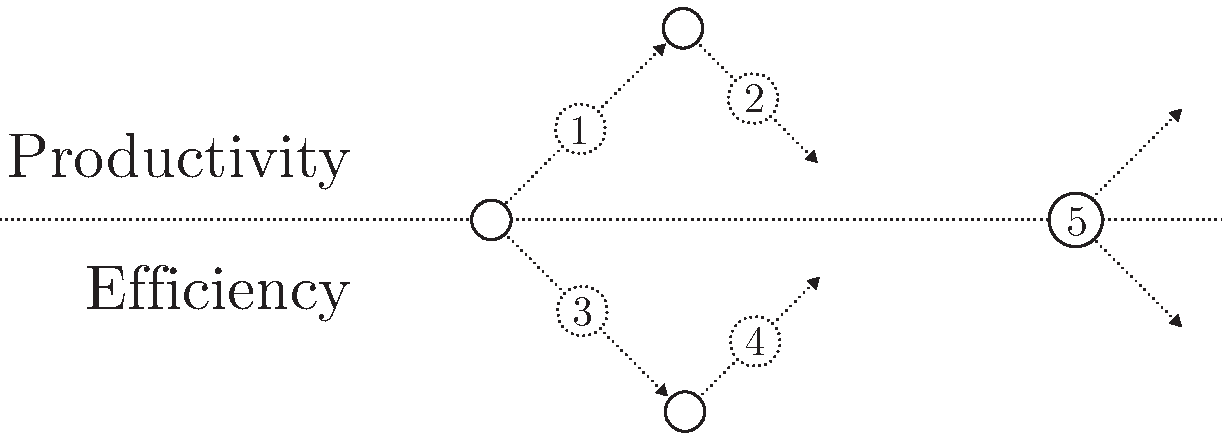
\includegraphics[width=0.6\textwidth]{../ressources/state-of-the-art.pdf}
\end{center}
\end{figure}

\subsection{Web Compliance}

TODO





\section{Software Maintainability} \label{chapter3:software-maintainability}

In order to improve and maintain a software system, it is important to holds in mind the mental representation behind its conception.
Architects, and mechanical engineers draw codified plans to share their mental representations with peers and building teams.
Similarly software developers write source codes.
But because the source code represents both the plan and its execution, the second aspect tends to shadow the first, and the mental representation is lost in technical details and optimizations.
It then becomes hard or even impossible to quickly grasp the purpose of the system without this mental representation.
Even the initial authors would have difficulties to understand the system after some times.
This problem becomes even more critical as the system grows in size.
Therefore, it is important to decompose the system into smaller subsystem easier to grasp individually.
Such decomposition improves the readability and comprehensibility hence maintainability of the implementation of a software system.
This section shows the theoretical tools for this decomposition, and their application in programming languages.


\subsection{Modularity}

\begin{center}
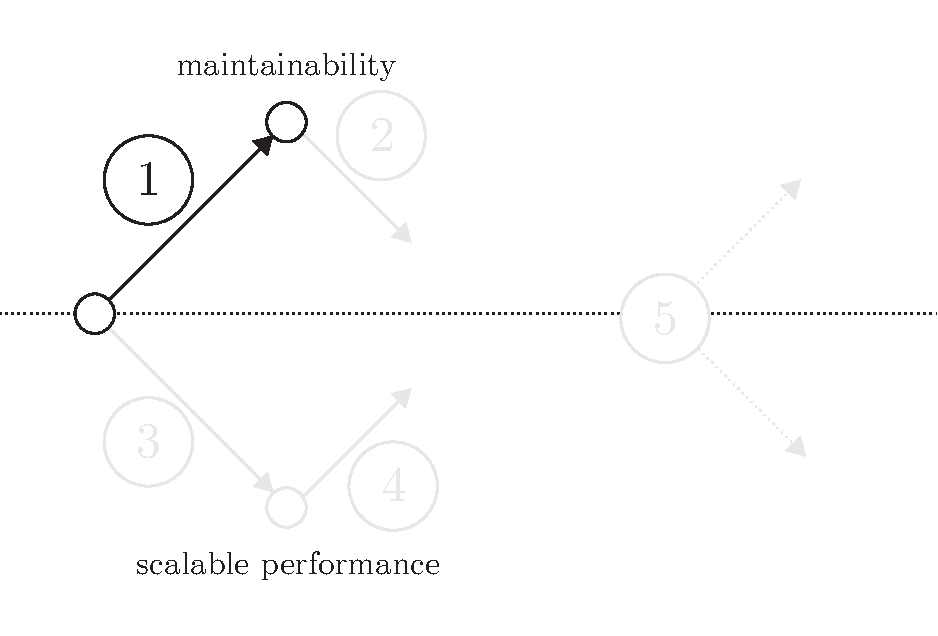
\includegraphics[width=0.6\textwidth]{../ressources/state-of-the-art-1.pdf}
\end{center}

\subsubsection{Design Choices}


\paragraph{Structured Programming}

\illustration{spaghetti programming}

The growing size and complexity of software systems eventually urges the developers to split the problem into isolated subproblems.
To respond to this problem, Dijkstra firstly developed the concept of Structured Programming \cite{Dijkstra1970}.
D. Knuth cited C. Hoare to define it as \textit{the systematic use of abstraction to control a mass of details, and also a means of documentation which aids program design} \cite{Knuth1974}.
Dijkstra formalized this procedure on two levels, at a fine grain and at a coarse grain \cite{Dijkstra1968a,Dijkstra1968}.

% A program expressed as a continuous flow of instructions with occasional jumps with 
The \texttt{goto} statement allows to jump anywhere in the code.
It makes the flow of control hard to follow and understand.
It is called spaghetti code.
Dijkstra advocated instead to decompose the implementation into structures and reusable functions to decompose the larger problem into many independent subproblems at a fine grain \cite{Dijkstra1968a}.
It is the precursor of many later programming trends.

\illustration{lasagna programming}

He also proposed to design complex systems with a hierarchical structure \cite{Dijkstra1968}.
It decomposes a system into layers at a coarser grain.
Each layer would abstract a design problem for the upper layers.
This work established grounds for what is know called modular programming.

% Letters to the editor : goto statement considered harmful \cite{Dijkstra1968a}
% The structure of the THE-multiprogramming system \cite{Dijkstra1968}

\paragraph{Modular Programming}

Modular programming advocates to design a software system as an assembly of modules communicating with each other.
The goal of using modular programming is twofold.
It allows to limit the understanding required to contribute to a module \cite{Stevens1974}.
% It allows a developer to limit its understanding only to the features isolated inside a module, instead of understanding the whole problem \cite{Stevens1974}.
And it reduces development time by allowing several developers to simultaneously implement different modules \cite{Wong2009,Cataldo2006}.

The criteria to decompose the system into well defined modules are coupling and cohesion \cite{Stevens1974}.
The coupling defines the strength of the interdependence between modules.
It is opposed to cohesion which defines how strongly the features inside a module are related.
Low coupling between modules and high cohesion inside modules imply a better readability and comprehensibility, hence a better maintainability of the implementation of the system.

These two criteria defines how modular is the implementation.
However, it doesn't define how well this organization will accept evolutions of the specification of the problem.
% stand against the evolution of the implementation.

% (See wikipedia page https://en.wikipedia.org/wiki/Separation_of_concerns)


\subsubsection{Design Choices}

The result of modular organization is that the modification on the implementation are easier to conduct within a module, than on the modules organization.
The impacts of the evolution of the problem should be concentrated as much as possible within the modules, and not in the modular organization, to reduce the overall impact on the implementation.
% It is important that the modular organization stand against the evolutions in the specification of the problem, and their consequences in the implementation.
% The interfaces between modules, and the contents of these modules need to be well thought.
The information hiding principle, and the separation of concerns are two similar approach to keep modifications within the modules.

\paragraph{Information Hiding Principle}

% helps define the content of modules so as to limit the impact of the evolution to a small portion of the implementation 
The information hiding principle advocates to encapsulate a specific design choice in each module to isolate the evolution on this choice from impacting the rest of the implementation \cite{Parnas1972}.
In this article, D. Parnas opposes the organization of modules following the information hiding principle from the one following a pipeline approach to parallelize the execution.
The former organization supports the development evolution, while the latter is more favorable to the performance of parallel execution.
This opposition shows that a program cannot trivially follow an organization that support both development evolution, and performance.
However, D. Parnas advocates the use of an assembler to conciliate the two approaches.

% The structure and value of modularity in software design \cite{Sullivan2001a}
% -> We identify an issue for software designers that neither Parnas’s formulation nor subsequent developments based on it adequately address: A designer is responsible for producing the greatest benefit for any given investment of time, talent, money, and other resources.

\paragraph{Separation of Concerns}

The Separation of Concern is a design principle advocating that each module is responsible for one and only one specific concern \cite{Tarr1999,Hursch1995}.
For example, the separation of the form and the content in HTML / CSS, or the OSI model for the network stack.
Each concern evolves independently without impacting the rest of the implementation.

However, this definition is orthogonal to the original meaning coined by Dijkstra \cite{Dijkstra1982}.
It is interesting to note this difference, as it is related directly to this thesis.
% Initially, it meant the ability to reason independently about different concern about a software system.
The initial definition was about analyzing independently how a system meets different concerns.
Dijkstra gives the example of analyzing independently correctness and efficiency.
It is impossible to encapsulate correctness, or efficiency in a module, they concern the whole system.
In this respect, this thesis is oriented towards dissociating the concern of development evolution and of performance.
That is to be able to reason on the maintainability of a program, independently than of its performance, and vice versa.
% This seems challenging as D. Parnas opposed these two concerns.
It is the challenge presented by D. Parnas when he opposed the two concerns in \cite{Parnas1972}.

This thesis investigates further this opposition to dissociate the concern of evolution and the concern of performance in the case of a web application.
The next section investigates the first concern, and presents the major programming models used to improve the evolution of an application.

\subsubsection{Programming Models} \label{chapter3:software-design:programming-models}

% Programming languages are designed for developers to follow the best practices mentioned above.
Programming languages used in the industry were designed following programming models favoring the use of the best practices mentioned above.
This section presents two programming models : object oriented programming and functional programming.

\paragraph{Object Oriented Programming}

% The following list defines Object-Oriented Programming (OOP).
% \begin{enumerate}
% \item Everything is an object.
% \item Communication is performed by objects communicating with each other, requesting that objects perform actions. Objects communicate by sending and receiving messages. A message is a request for action, bundled with whatever objects may be necessary to complete the task.
% \item Objects have their own memory, which consists of other objects.
% \item Every object is an instance of a class. A class simply represents a grouping of similar objects, such as integers or lists.
% \item The class is the repository for behavior associated with an object. That is, all objects that are instances of the same class can perform the same actions.
% \end{enumerate}

Alan Kay, who coined the term, states that Object Oriented Programming (OOP) is about message-passing, encapsulation and late binding.
(There is no academic reference for that, only a public mail exchange\ftnt{http://userpage.fu-berlin.de/~ram/pub/pub\_jf47ht81Ht/doc\_kay\_oop\_en}.)
This original definition is an evolution upon modular programming.
It helps encapsulate both the data, and the functions to process this data in an isolated, loosely coupled module.
The very first OOP language was Smalltalk \cite{Goldberg1984}.
It defined the core concept of OOP.
It is inspired by LISP and by the definition of the Actor Model, which we will define in the next section.

% Illustration of multiple cells, as Alan Kay thought of biology when developing the object-oriented concepts.
% http://userpage.fu-berlin.de/~ram/pub/pub_jf47ht81Ht/doc_kay_oop_en
% I thought of objects being like biological cells [...] able to communicate with messages ...

Object-Oriented Programming abandoned late-binding and adopted a stricter approach with the concepts of class, inheritance and polymorphism.
The major languages of the software industry feature this stricter Object-Oriented approach.
We can cite C++ and Java as the emblematic figures of OOP \cite{Gosling2000,Stroustrup1986}.

Though, the field test seems to have had reason of this stricter version.
The trends in programming language seems to digress from the pure Object-Oriented approach to evolve toward a more dynamic approach, closer to Functional Programming.
Indeed Javascript, Ruby and Python adopt functional features such as dynamic typing and higher-order functions \cite{Ecma1999}\ftnt{https://www.ruby-lang.org/en/about/}.

% \paragraph{Object Calisthenics}

% Object calisthenics are defined as the chapter 6 of \textit{The Thoughtworks Anthology} \cite{Bay2008}.
% It is an exercise for developers presented as a list of 9 rules to follow to enforce maintainability and readability on source code \ftnt{http://www.cs.helsinki.fi/u/luontola/tdd-2009/ext/ObjectCalisthenics.pdf}.

% Some of these rules are direct implementations of the more general concept of separation of concerns, and information hiding.
% As an example, rule 7 \textit{Keep all entities small} advocate that entities should have a concise concern.
% Other rules are just syntactic guides to improve readability and comprehensibility.


% See Object calisthenics 
% - http://williamdurand.fr/2013/06/03/object-calisthenics/
% - http://www.cs.helsinki.fi/u/luontola/tdd-2009/ext/ObjectCalisthenics.pdf



\paragraph{Functional Programming} \label{chapter3:software-design:programming-models:functional-programming}

% \cit{All problems in computer science can be solved by another level of indirection}{Butler Lampson}

The formal definition of Functional Programming resides in manipulating only mathematical expressions - instead of operation statements - and forbidding state mutability.
However, the functional programming concepts implemented in programming language are more mitigated, and resides in higher-order functions and lazy evaluation.
Two features that major programming languages now commonly present.
Higher-order functions and lazy evaluation help loosen the couple between modules, and improve their re-usability.
\textit{In fine}, it helps developers to write applications that are more maintainable, and favorable to evolution \cite{Hughes1989}.

\paragraph{Higher-Order Function}

Languages providing higher-order functions allows to manipulate functions like any other primary value : to store them in variables, or to pass them as arguments.
Higher-order functions replace the needs for most modern object oriented programming design patterns \ftnt{http://stackoverflow.com/a/5797892/933670}.

\paragraph{Closures}

Most languages use closures to implement lexical scope with higher-order functions \cite{Sussman1998}.
A closure is the association of a function and the lexical context from its creation.
It allows this function to access variable from this context, even when invoked outside the scope of this context.
For example when passed as an argument to another module.

It loosen the couple between modules, and helps define more generic and reusable modules.
However, it increase their dependencies during the execution.
Indeed, by exchanging closures, two modules intricately share their contexts of execution.

\paragraph{}

Functional programming greatly improves the resilience of implementation to the evolution of their specification.
However, it requires a global memory to share the context of execution among modules.
The next section shows that sharing memory makes parallelism difficult.
At the regard of this insight, the concern of evolution and the concern of performance seem hardly compatible.


\subsubsection{Higher-Order Programming}

\nt{TODO higher-order programming and modularity}

\subsubsection{Limitations}

\nt{TODO Transition on the limitations of software modularity}

\subsection{Performance Improvements}

\begin{center}
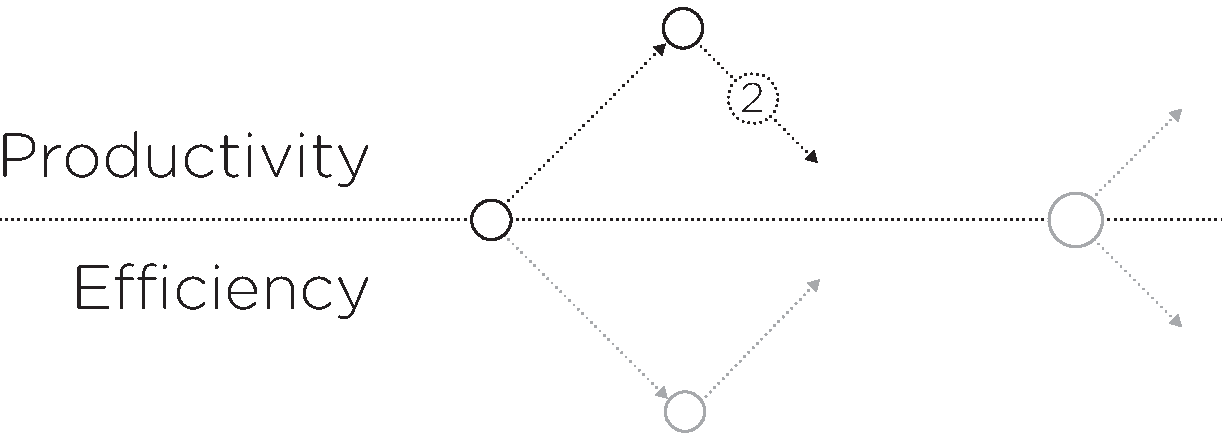
\includegraphics[width=0.6\textwidth]{../ressources/state-of-the-art-2.pdf}
\end{center}

\subsubsection{Compilation}


% Instead of trying to find a fitting between the two organization,
Another approach to conciliate performance and maintainability, is to transform the source from one organization into the other.
\textit{It is a mistake to attempt high concurrency without help from the compiler} \cite{Behren2003}.
When showing the incompatibility between the two organization, D. Parnas already advocated conciling the two methods using an assembler to transform the development organization into the execution organization \cite{Parnas1972}.
I present in the this section the state of the art in compilation-based parallelization.

% Imperative Stream Processing
%   Piccolo                                  Parallel in-memory \cite{Power2010}
%   CIEL                                    Stateless dataflow \cite{Murray2011}
%   Statdeful Dataflow Graph (SDG)          Stateful dataflow  \cite{Fernandez2014a}

\paragraph{Parallelism Extraction}

Generally, there is three type of parallelism, data, task and pipeline parallelism.
Some works explore the extraction of the three types indistincly \cite{Li2012}.
Other works focused on the task parallelism \cite{Rinard1996}.
However, huge works has been done on the data parallelization, to parallelize the loops inside a sequential program \cite{Mauras1989,Amarasinghe1995,Yuki2013,Banerjee2013,Radoi2014}
Indeed, the loops represent most of the execution time in scientific applications, so an important speedup is expected from this data parallelization.
C. Hermann studied the parallelization of loop in a functional language with higher-order programming and immutable data \cite{Herrmann2000}.
However, there is few works to parallelize higher-order programming languages, with mutable data.
Closures often complicates the dependencies between iterations.
To conserve higher-order programming, N. Matsakis proposed to forbid the mutation of the parent closure of a loop, so that the iterations can be executed in parallel while accessing the immutable closure\cite{Matsakis2012a}.

All these approaches are based on synchronous execution and Amdahl's law states that even if a slight portion of execution is sequential, the expected speedup is limited \cite{Amdahl1967,Clements2013a}.
Another approach to break free from the sequential structure is to split the sequential execution into following, parallelizable tasks to form a pipeline \cite{Kamruzzaman2013,Fernandez2014a}.
This thesis focus solely on pipeline parallelism.

Pipeline parallelism is relevant for multi-pass algorithms \cite{Conway1963}, and it is particularly efficient for stream processing applications as we saw in section \ref{chapter3:software-efficiency:dataflow-pipeline}.
For these applications, sequentiality is no longer relevant, as the different stages of the execution are repeated for each message in the stream.
Only causality is necessary, and it opens a possible pipeline parallelism.


\paragraph{Static analysis}

In order to extract parallelism, compilers analyze the source code of applications.
The compiler analyzes the control flow to detect the dependencies between statements to parallelize them.
As these dependencies are linked to memory access, it is important to have a good memory representation.
The point-to analysis, presented by L. Andersen \cite{Andersen1994} is a common approach to extract the memory representation.
It analyzes the modification of pointers through the control flow, to help extract properties from programs.
It is used in security to assure the safeness of an implementation, for example in Javascript \cite{Chudnov2015}.
% However, these techniques are not precise enough to rely only on them for the parallelization.

\paragraph{Annotations}

Extracting parallel dataflow from an imperative, sequential implementation is a hard problem \cite{Johnston2004a}.
Some works proposed to rely on annotations from the developer to help the extraction \cite{Vandierendonck2010a,Fernandez2014a}.
% Some works asked the developers to annotate their code so as help the compiler extract parallelism
% It is an intermediate solution with the solution presented in the previous section.
However, it still requires developers indicate the independence of the memory or the execution.
In this regard, this solution is similar to concurrent programming present in \ref{chapter3:concurrent-programming}, and are unable to fix the rupture between performance and maintainability.

All the solution presented throughout this chapter are elitist, as they tend to rely on the developer to reconcile the two organizations.
They are not satisfactory as they are too hardly accessible for most developers.
It finally results in frail implementations, that require great efforts of development to assure their performance in the first place, and then to maintain.

\subsubsection{Concurrent Programming}

\nt{TODO Event-loop / event-based programming / concurrent programming}

\begin{center}
\rule{3cm}{0.4pt}
need integration
\rule{3cm}{0.4pt}
\end{center}

\paragraph{Interdependencies}

It is easy to understand the parallelism in a cooking recipe because the interdependencies between operations are trivial.
It seems obvious that melting chocolate is independent from whipping up egg whites.
% Because chocolate and egg whites are different ingredients.
This distinction between chocolate and egg whites is trivial.
% ... comes from the modifications to the state.
While the distinctions within the state of an application are more intricate.
This makes concurrent application more difficult to design and implement.

\subparagraph{State Coordination}

% The interdependencies between the tasks impose the coordination of the global application state.
The global state of an application impose the coordination between the tasks.
This coordination happens either by sending messages, or by modifying a shared memory.
\nt{The following sentence needs to be rewritten to include both message passing and shared memory. Because state coordination limits parallelism, and scalability, it is a better solution to use message passing}
If the tasks are independent enough, the coordinations can be done with message passing.
Each task sends messages to indicate the modifications of the state with consequences outside its scope.
% They pass the states from one task to another so as to always have an exclusive access on the state.
% As example, applications built around a pipeline architecture define independent tasks arranged to be executed one after the other.
% The tasks pass the result of their computation to the next.
% These tasks never share a state.
However, if the tasks are too dependent, the overhead of message passing tends to impact performances.
% If the tasks need concurrent accesses to a state, they cannot efficiently pass the state from one to the other repeatedly.
They need to share and coordinate their accesses to the state.
Each access needs to be exclusive to avoid corruption.
I address in the next paragraphs the different scheduling strategies, and how they assure this exclusivity.

\subparagraph{Task Scheduling}

There are two scheduling strategies to execute tasks sequentially on a single processing unit : preemptive scheduling and cooperative scheduling.
The coordination is different with the two scheduling strategies.

\illustration{feu rouge et rond point}

Preemptive scheduling is used to assure fairness between the tasks, such as in a multi-tasking operating system.
% in most execution environment in conjunction with multi-threading.
The scheduler allows a limited time of execution for each task, before preempting it.
% It is a fair and pessimistic scheduling, as it grant the same amount of computing time to each task.
However, as the preemption happens unexpectedly, the developer needs to assure exclusivity by locking the shared state before access.
Locking is known to be hard to manage by developers, and to impact performances negatively.
Because it is not ideal both for development scalability and performance scalability, it is set aside for the remaining of this chapter.
% This scheduling strategy should be avoided except when true concurrency is needed in concert with true shared state.
% Shared state could probably always be emulated with isolated memory and message passing.

On the other hand, in cooperative scheduling, a task is allowed to run until it yields the execution back to the scheduler.
Each task is an atomic execution : it has an exclusive access on the memory.
% It gives back to the developer the control over the preemption.
As the developer doesn't need to explicitly assure exclusivity, it is easier to write concurrent programs efficiently with this scheduling strategy.
% Indeed, I presented in the previous section the popularity of Javascript, which is often implemented on top of this scheduling strategy (DOM, Node.js).

\subparagraph{Invariance}

\nt{TODO This section is not clear. It should be moved in the state of the art.}

% The challenge introduced above is to assure to the developer an exclusive access to the state of its application.
In concurrent computation, it is important to assure the invariance of a state during its manipulation.
This assurance is given by the exclusive access of an atomic execution on the state.
% I call invariance the assurance given that the state accessible from a task will remain unchanged during its access to avoid corruption, and more generally to allow the developer to perform atomic modifications on the state.
It allows the developer to group operations inside this atomic execution, so as to avoid corruption of the state.
% so as to perform all the operations without interference from concurrent executions.
% The same concept is found in transactional memory.

When the tasks remains isolated and communicate by message passing, there is no risk of corrupted state.
The invariance is assured by the isolation of the state specified by the developer, and by the atomicity of the message processing.
On the other hand, in a cooperative scheduling application, each task is atomic, so the developer always has an exclusive access to the global state.
This atomicity assures the invariance.
% The invariance is assured by the atomicity of each task.
% , because any region in the memory can be accessed only by one task at a time.

% Between these two invariances, the locking mechanisms seems to be a promising compromise.
% The developer defines only the shared states, and these are locked only when needed.
% However, it increases the complexity of the possible locked combination, leading to unpredictable situations, such as deadlock, and so on.
% The locking mechanisms are known to be difficult to manage, and sub-optimal.
% Indeed, they are eventually as efficient as a queue to share resources.

% For the rest of this thesis, I focus only on the invariances provided by the multi-process paradigm and the cooperative scheduling.
% They two invariance are similar, because the developer defines sequence of instructions with atomic access to the memory.
% And in both paradigms, these sequences communicate by sending messages to each other.
The difference is that in the message passing paradigm, the developer defines the state isolation inducing the execution isolation, while with cooperative scheduling, the developer defines only the execution isolation.
% This difference seems to be crucial in the adoption by the developer community.
It is difficult for developer to isolate state, but it provides good performances through parallelism.
While it is easier to assure atomic execution with cooperative scheduling, but it is unable to provide parallelism.
On one hand, the state is distributed and isolated to improve performance scalability.
On the other hand, the code is organized logically to improve maintainability.
The impact of these two organizations on performance scalability and development scalability is at the heart of this thesis.

\begin{center}
\rule{3cm}{0.4pt}
end integration
\rule{3cm}{0.4pt}
\end{center}


\subsubsection{Limitations on Accessibility}

\paragraph{Transition on parallel programming}

\endinput

\subsubsection{Modularity based on Design Decisions}

Designing Software for ease of extension and contraction \cite{Parnas1979}

Design Rules: The Power of Modularity Volume 1 \cite{Baldwin1999}
A reference book, but I can't get it.


Promises 
\cite{Liskov1988}


What makes a great software engineer? \cite{Li2015}

About great software development:
Productivity : Sackman et. al 68, Gugerty & Olson 86
Collaboration, meaningful contribution : Kelly 99, Begel & Simon 06, Hewner & Guzdial 10
Communicate and acquire understanding : LaToza 06, Ko 06
Technical Knowledge : 
Open minded : McConnell 04, Bryant 13




Modularity :
- encapsulation : a module contains the data, as well as the functions to manipulate this data
- separation of concerns : each module should have a clear scope of action, and this scope should not overlap with the scope of other modules
- loose coupling : each module should require no, or as little knowledge as possible about the definition of other modules






Continuations and coroutines \cite{Haynes1984}
-> THIS

Parallel closures, a new twist on an old idea \cite{Matsakis2012a}

Continuation of work on SEDA \cite{Salmito2014}



From control flow to dataflow \cite{Beck1991}


-> THIS, to read
Automatic Extraction of Coarse-Grained Data-Flow Threads from Imperative Programs \cite{Li2012}
In this paper all parallelism are extracted (data, task and pipeline).


Commutativity analysis: A new analysis framework for parallelizing compilers \cite{Rinard1996}
In this paper, they analyze commutative operations to parallelize them.
It is novel because it isn't about parallelizing loops.
However, it is not exactly pipeline parallelism either.


Interesting articles :

http://comjnl.oxfordjournals.org/content/early/2015/09/15/comjnl.bxv077.abstract


-> THIS, to read
Load balanced pipeline parallelism \cite{Kamruzzaman2013}


??? The Paralax infrastructure \cite{Vandierendonck2010a}

??? Blazes: Coordination analysis for distributed programs \cite{Alvaro2014}

Making state explicit ... \cite{Fernandez2014a}
http://2015.splashcon.org/event/splash2015-splash-i-lindsey-kuper-talk


Introducing 'Bones': a parallelizing source-to-source compiler based on algorithmic skeletons \cite{Nugteren2012}


Recent paper about Javascrypt static analysis \cite{Chudnov2015}



Loop nesting optimization
- systolic arrays
- polyhedral compilers
- Simplifying reductions 


\cite{Mendis2015}
\section{Performance Efficiency Focused Environements} \label{chapter3:software-performance}

With the limitations on performance presented in the previous section, both academy and industry communities proposed alternative solutions with performance in mind.
Section \ref{chapter3:software-performance:concurrency} presents the concurrent and parallel programming paradigms, and their programming models. % oriented on performance rather than maintainability.
Section \ref{chapter3:software-performance:adoption} presents the adoption steered by the performance efficiency of parallel programming.
Section \ref{chapter3:software-performance:maintainability-limitations} presents the consequences of parallelism on maintainability.
Finally, section \ref{chapter3:software-performance:summary} summarizes the three previous sections in a table.

\subsection{Concurrency} \label{chapter3:software-performance:concurrency}

\begin{figure}[h!]
\begin{center}
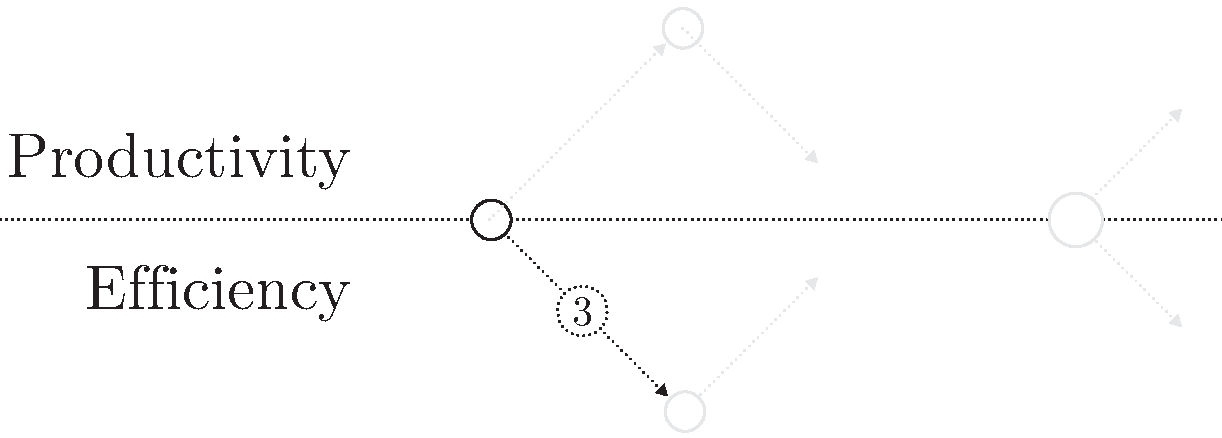
\includegraphics[width=0.6\textwidth]{../ressources/state-of-the-art-3.pdf}
\end{center}
\caption{}
\label{fig:state-of-the-art-3}
\end{figure}

Web servers need to be able to process huge amount of concurrent operations in a scalable fashion.
Concurrency is the ability to make progress on several operations roughly simultaneously.
It implies to draw boundaries in the memory to define independent regions, and causality in the execution to define independent tasks.
When both boundaries and causality are clearly defined, the tasks can be scheduled in parallel to make progress strictly simultaneously.

The definition of independent tasks allows the fine level synchronization within a task, and coarse level message passing between the tasks required for performence efficiency.
The synchronization of execution at a fine level assures the invariance on the shared state, and avoid communication overhead.
The message-passing at a coarser level assures the parallelism.
The two are indispensable for performance efficiency.

\subsubsection{Concurrent Programming} \label{chapter3:software-maintainability:concurrency:concurrent-programming}

% \cit{Building concurrent programming is like building a steam engine through a keyhole}{TODO}

\illustration{feu rouge et rond point}
Concurrent programming provides the mechanisms to define the causality of execution and assure the invariance of the global memory.
There are two scheduling strategies to execute tasks sequentially on a single processing unit, cooperative scheduling and preemptive scheduling.

\begin{description}
\item[Cooperative Scheduling] allows a concurrent execution to run until it yields back to the scheduler.
Each concurrent execution has an atomic, exclusive access on the memory.
\item[Preemptive Scheduling] allows a limited time of execution for each concurrent execution, before preempting it.
It assures fairness between the tasks, such as in a multi-tasking operating system.
But the unexpected preemption breaks atomicity, the developer needs to lock the shared state to assure atomicity and exclusivity.
\end{description}

The next paragraphs presents the event-driven programing model, based on cooperative scheduling, and the multi-threading programming model, based on preemptive scheduling.
Additionally, they present lock-free data-structures, which is independent from the scheduling strategy, as they rely on atomic memory operations.

\paragraph{Event-Driven Programming}

Event-driven execution model queues explicitly defined concurrent tasks needing access to shared resources.
The concurrent tasks are schedule sequentially to assure exclusivity, and cooperatively to assure atomicity.
% Web servers needs to be highly concurrent, and efficient.
It is very efficient for highly concurrent applications, as it avoids contention due to waiting for shared resources like disks, or network.
Several execution model rely on this execution model, like TAME \cite{Krohn2007}, Node.js\ftnt{https://nodejs.org/en/} and Vert.X\ftnt{http://vertx.io/}.
As well as some web servers like Flash \cite{Pai1999}, Ninja \cite{Gribble2001} thttpd\ftnt{http://acme.com/software/thttpd/} and Nginx\ftnt{https://www.nginx.com/}.

% However, a drawback of this model was that the execution context is lost at each event.
% The developer needs to explicitly transfer the relevant state to continue the execution from one event execution to another.

% + Fibers \cite{Adya2002}
% + Capricio \cite{Behren2003a} - User cooperative threads (also known as fibers / green threads)

% The problem of losing the execution context disappears with closures in higher-order programming.
% \nt{link with the previous paragraph}
% Moreover, the continuation passing style used in higher-order programming requires the developer to be aware of the asynchronous rupture in the execution, so as to assure atomicity \cite{Sussman1998}.
% And because an asynchronous call doesn't wait for the completion of the operation, the asynchronous control flow is not limited to be linear like in threads. \nt{more about that}
% Multiple asynchronous calls are made in parallel.

% + TAME \cite{Krohn2007} - event-based solution without stack ripping in C (it is like closure, but for C)
% + Node.js - \ftnt{https://nodejs.org/en/}
% + Vert.X - \ftnt{http://vertx.io/} node like + thread / worker capabilities

But the event-driven model is limited in performance.
The concurrent tasks share the same memory, and cannot be scheduled in parallel.
The next paragraph present work intending to improve performance. % by reducing the sequential portions to a minimum to increase the possibilities of parallelism.

\paragraph{Lock-Free Data-Structures}

The wait-free and lock-free data-structures reduce the exclusive execution to a minimum of instructions \cite{Lamport1977,Herlihy1988,Herlihy1990,Herlihy1991,Anderson1990}.
They arrange these instructions into small atomic operations to avoid the need to lock.
They are based on atomic read and write operations provided by transactional memories \cite{Harris2010}.
They provide concurrent implementation of basic data-structures such as linked list \cite{Valois1995,Timnat2012}, queue \cite{Sundell2003,Wimmer2015}, tree \cite{Ramachandran2015} or stack \cite{Hendler2004}.

However these atomic operations are uncommon hence difficult to develop with.
The next paragraph present the multi-threading improving parallelism with explicit synchronization from the developer.
% using coarser granularity of atomic execution and exclusivity.

% Reference papers :
% Concurrent reading and writing \cite{Lamport1977}
% Impossibility and universality results for wait-free synchronization \cite{Herlihy1988}
% A methodology for implementing highly concurrent data structures \cite{Herlihy1990}
% Wait-free synchronization \cite{Herlihy1991}

% Book :
% The virtue of Patience: Concurrent Programming With And Without Waiting \cite{Anderson1990}

\paragraph{Multi-Threading Programming}

Threads are light processes sharing the same memory execution context within an isolated process \cite{Dijkstra1968}, and scheduled in parallel with fork/join operations \cite{Randall1998,Frigo1998,Leiserson2010}.
They execute statements sequentially waiting for completion, and are scheduled preemptively to avoid blocking the global progression.
The preemption breaks the atomicity of the execution, and the parallel execution breaks the exclusivity of memory accesses.
To restore atomicity and exclusivity, hence assure the invariance, multi-threading programming models provide synchronization mechanisms, such as semaphores \cite{Dijkstra}, guarded commands \cite{Dijkstra1975}, guarded region \cite{Hansen1978a} or monitors \cite{Hoare1974}.

Developers tend to use the global memory extensively, and threads require to protect each and every shared memory cell.
This heavy need for synchronization leads to bad performances, and is difficult to develop with \cite{Adya2002}.

\paragraph{Fibers}

Cooperative threads, or fibers proposed to join the advantage of threads sequentiality, with the advantage of cooperative scheduling \cite{Adya2002,Behren2003a}.
It avoids splitting the execution into atomic tasks nor use synchronization mechanisms to protect the memory.
A fiber yields the execution to another fiber for a long-waiting operation to avoid blocking the execution, and recovers it at the same point when the operation finishes.

However, developers need to be aware of these yielding operation to preserve the atomicity\ftnt{https://glyph.twistedmatrix.com/2014/02/unyielding.html}.

\paragraph{}

The table \ref{tab:performance-concurrency} presents a summary of the analysis of performance of the platforms presented in this section.

\begin{table}[h!]
\small
\begin{tabu} to \linewidth {@{} l X[l] c c c c @{}}
%
% \multicolumn{3}{c}{}  & \lab{Concurrency} & \multicolumn{2}{|c}{Parallelism} \\
Model & Implementations    & \lab{Fine level sequentiality} & \lab{Coarse level message passing} & $\to$ & \lab{Performance Efficiency} \\
\tabucline[.5pt]{-}
%                                                                               SEQ  MSG   SCL
Event-driven programming       & Node.js, Vert.X                               & \V & \X && \X \\ \tabucline[on .5pt]{-}
Lock-free Data Structures      &                                               & \V & \X && \X \\ \tabucline[on .5pt]{-}
Multi-threading programming    & Lock, Mutex, Semaphores, Guarded regions      & \V & \X && \X \\ \tabucline[on .5pt]{-}
Cooperative threads            & Fibers                                        & \V & \X && \X \\
\tabucline[.5pt]{-}
\end{tabu}
\caption{Analysis of the state of the art in concurrent programming regarding performance efficiency}
\label{tab:performance-concurrency}
\end{table}


\paragraph{Performance Limitation of Concurrent Programming}



% Moore's law \cite{Moore1965} which forecasts the density of transistors per processing unit, was wrongly interpreted to promise the exponential evolution in the sequential performance of the processing unit, and the assurance for the software industry of always faster hardware.
% But as transistors attained a critical size, the reduction in power required by transistor predicted by the Dennard's MOSFET scaling \cite{Dennard2007} stopped\ftnt{https://cartesianproduct.wordpress.com/2013/04/15/the-end-of-dennard-scaling/}.

The total ordering imposed by fork/join threads is excessive.
The causal ordering proposed by the event-driven execution model is sufficient to assure correctness of a concurrent system \cite{Lamport1978,Reed2012}.
But because of the lack of clear isolation of the memory, the execution is not parallel, hence the performance is limited.
Synchronization mechanisms define shared memory, and lock-free data structures improve the parallel portion of execution, but the performance remains limited.
Parallel programming is the only solution for performance efficiency, at the expense of development efforts to explicitely define the memory isolation of concurrent tasks.

% Concurrent programming is a compromise to process operations simultaneously, by introduction synchronization to assure the exclusion required for shared states.


% The ever growing number of transistor predicted by Moore's law \cite{Moore1965} are arranged in parallel architecture to continue increasing the performance of processing units.
% Parallel programming became the only solution for performance efficiency, at the expense of development effort.


% This section presents the parallel programming solutions and their limitations in accessibility, and then the improvements to overcome these limitations.


% \nt{The shared-nothing architecture \cite{Stonebraker1986}}


\subsubsection{Parallel Programming} \label{chapter3:software-performance:parallel-programming}


Concurrent programming is based on the causal ordering of execution.
% The ordering of operations is local within a synchronous execution, while the concurrent executions are causally ordered.
% It leads to parallel execution with some coordinations such as synchronization, immutability or isolation.
With isolation of their memory, concurrent tasks can be scheduled in parallel.

This section presents the theoretical and programming models based on asynchronous communication and isolated execution for parallel programming.
It then presents with stream processing programming model.
And finally,it concludes on the limitations of parallel programming regarding maintainability. 

\nt{read and include \cite{Asanovic2006}}

\paragraph{Asynchronous and Isolated Process Parallelism}

The Flynn's taxonomy \cite{Flynn1972} is the most commonly used to categorize parallel execution.
It separates the flow of instructions, and the flow of data ; each being unique, or multiple.
All the current parallel programming model currently belong to the category Multiple Instruction Multiple Data (MIMD), which is further divided into Single Program Multiple Data (SPMD) \cite{Auguin1983,Darema1988,Darema2001} and Multiple Program Multiple Data (MPMD) \cite{Chang1997,Chan2004}.
MIMD implies several threads of execution processing several stream of data.
% The difference between SPMD and MPMD holds on the distinction of instruction pool between the threads of execution.
% SPMD implies to replicate the same program on all the processing units, while MPMD implies to define different programs for every processing units.

\begin{figure}
\begin{center}
\includegraphics[width=0.2\textwidth]{../ressources/SISD.pdf}
\includegraphics[width=0.2\textwidth]{../ressources/SIMD.pdf}
\includegraphics[width=0.2\textwidth]{../ressources/MISD.pdf}
\includegraphics[width=0.2\textwidth]{../ressources/MIMD.pdf}\\
by I, Cburnett. Licensed under CC BY-SA 3.0 via Commons
\url{https://commons.wikimedia.org/wiki/File:{SISD,SIMD,MISD,MIMD}.svg}
\end{center}
\caption{Flynn's taxonomy of parallelism}
\label{fig:flynn-taxonomy}
\end{figure}


The difference between SPMD and MPMD is in the representation of the execution in implementation.
SPMD organizes the implementation as a single execution replicated on many processing units.
While MPMD organizes explicitly the different threads of execution in the implementation.
Examples of SPMD programming languages are
Split-C \cite{Culler},
CRL \cite{Johnson1995} and
Composite C++ \cite{K.ManiChandy2005}.
%
Examples of MPMD programming languages are
Mentat \cite{Grimshaw1991},
Fortran M \cite{Foster1995b} and
Nexus \cite{Foster1996}.

% SPMD is close to the model presenting parallel improvements over modular programming presented in section \ref{chapter3:software-maintainability:programming-models}.
% While MPMD is closer to the programming models based on isolated process presented in the remaining of this section.
The coordinations between these threads of execution were done by message passing, using PVM \cite{Sunderam1994}, MPI \cite{Snir1996,Walker1996}, SOAP, or the more recent REST protocols.

\paragraph{Theoretical Models}

The total ordering of execution imposed by sequential execution is an overkill.
The causal ordering is sufficient to assure correctness in a distributed system \cite{Lamport1978,Reed2012}.
% As Lamport showed \cite{Lamport1978}, and Reed related later \cite{Reed2012}, causal order is sufficient to execute correctly a system in parallel, such as a distributed system.
% The total ordering of execution provided by synchronization is an overkill.
Moreover, the communication in reality are subject to various faults and attacks \cite{Lamport1982} and too slow compared to execution to be synchronous.
The Actor model is one of the first programming model to be explicitly designed to take these physical limitations in account \cite{Hewitt1977a}.
It allows to express the computation as a set of communicating actors \cite{Hewitt1973a, Hewitt1977, Clinger1981}.
In reaction to a received message, an actor can create other actors, send messages, and choose how to respond to the next message.
All actors are executed concurrently, and communicate asynchronously.
An asynchronous communication implies that the sender continues its execution immediately after sending the message, before receiving the result of the initiated communication.

In the Actor Model, everything is an actor, even the simplest types like numbers.
This level of granularity is unachievable in practice due to overhead from the asynchronous communications.
Most implementations adopt a granularity on the process or function level.

Coroutines are autonomous programs which communicate with adjacent modules as if they were input and output subroutines \cite{Conway1963}.
It is the first definition of a pipeline to implement multi-pass algorithms.
Similar works include the Communicating Sequential Processes (CSP) \cite{Hoare1978, Brookes1984}, and the Kahn Networks \cite{Kahn1974, Kahn1976}.


\paragraph{}

Table \ref{scalability-actor-model} presents a summary of the analysis of the paradigm presented in the previous paragraphs.

\begin{table}[h!]
\label{scalability-actor-model}
\small
\begin{tabu} to \linewidth {@{} l X[l] c c c c @{}}
%
% \multicolumn{3}{c}{}  & \lab{Concurrency} & \multicolumn{2}{|c}{Parallelism} \\
Model & Implementations    & \lab{Fine level sequentiality} & \lab{Coarse level message passing} & $\to$ & \lab{Performance Efficiency} \\
\tabucline[.5pt]{-}
%                                                                               SEQ  MSG   SCL
Event-driven programming       & Node.js, Vert.X                               & \V & \X && \X \\ \tabucline[on .5pt]{-}
Lock-free Data Structures      &                                               & \V & \X && \X \\ \tabucline[on .5pt]{-}
Multi-threading programming    & Lock, Mutex, Semaphores, Guarded regions      & \V & \X && \X \\ \tabucline[on .5pt]{-}
Cooperative threads            & Fibers                                        & \V & \X && \X \\
\tabucline[.5pt]{-}
Actor Model                    & Scala, Akka, Play, Erlang                     & \V & \V && \V \\
\tabucline[.5pt]{-}
\end{tabu}
\caption{Analysis of the state of the art in concurrent and parallel programming regarding performance}
\end{table}





\subsection{Adoption} \label{chapter3:software-performance:adoption}

\begin{figure}[h!]
\begin{center}
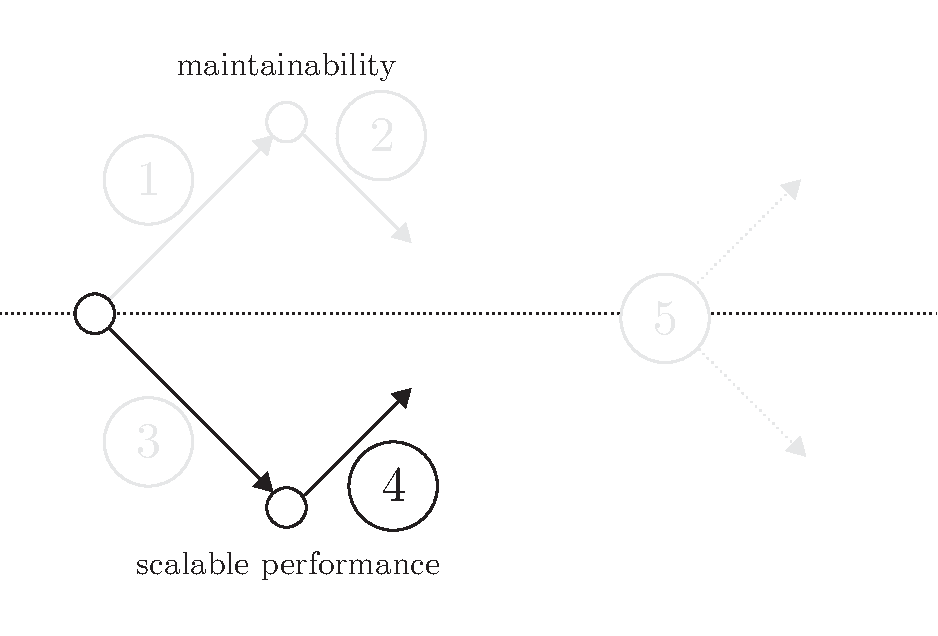
\includegraphics[width=0.6\textwidth]{../ressources/state-of-the-art-4.pdf}
\end{center}
\caption{}
\label{fig:state-of-the-art-4}
\end{figure}

The performance improvements comes directly from the industry requirements.
All these system make sens in industrial context, even the smallest.
When the need for performance is higher than the need for maintainability, the research merges with the academy.
% Industries have the money to fund the necessary research.
If there is industrial need, there will be maintenance.
The languages on the Mars Rover or in banking systems are 30 years old, and there is no community to maintain it.
Yet the industry continue to maintain these languages.

However, the context of this thesis is different from a classical industrial context.
During the bootstrap of a web application project, the economical context requires technologies with strong community, to pick talents from to grow the team quickly and effortlessly.
It also requires these technologies to be of industrial standard, to build a reliable product.
And these technology must be compatible with web technologies.

The context of this thesis requires the technology to meet all the three criteria.
\begin{itemize}
\item Community support
\item Industrial need
\end{itemize}


\nt{review this paragraph and the transition to the next section}
The field of concurrent programming is so vast it is impossible to relate here every programming languages.
The previous examples are only the best known.
The next focus focuses on streaming real-time applications.

% \comment{transition on lazy evaluation equivalence to stream. lazy evaluation + side effects + concurrency = streams}



% + all the solutions that have a great industrial impact (storm, millwheel and co)



\subsubsection{Exection Decomposition}


The programming paradigms presented above are implemented in many existing programming languages.
All major programming languages implements some form of concurrency or parallelism mechanism.
The next paragraphs presents these implementations by the industry and the community.
And more specifically, how they deal with the need to decompose the execution.

\paragraph{Event-Loop}

The event-loop model, featured by the DOM and Node.js with Javascript, allows concurrency but not parallelism.
It decomposes the execution into sequences of callbacks functions, but keep the memory shared.

As presented in the previous section, Javascript is currently one of the most used language.
This asynchronous programming model without the memory decomposition seems to be easy to develop with.
It is used extensively in the community as well as in the industry.
However, when the programming model requires the memory to be decompose, in order to get parallelism, it becomes more complicated to develop with, as presented in the next paragraphs.

\paragraph{Multi-Threading}

The multi-threading model allows concurrency and parallelism on certain execution region.
It decomposes the execution into fork-join threads, and the memory is shared, but protected with locks.
The protection of the shared memory is the reason concurrent programming is difficult to manage for most developers.
Multi-threading is difficult to program with, and for this reason, it leads to poor performances.
It is not heavily used in the community, where the need for concurrency is limited.
In the industry, where the concurrency is often required, multi-threading is abandoned for other paradigms, such as the event loop or the actor model.

\paragraph{}

The event-loop requires an execution decomposition, but not a memory decomposition.
This paradigm is heavily adopted by both the community and the industry.
On the other hand, the multi-threading paradigms with locks requires an execution decomposition, and light memory decomposition.
This paradigms is not heavily used in the community, and is being abandoned by the industry.
This comparison between the event-loop and the multi-threading paradigms seems to indicate that the memory decomposition heavily restrains the adoption by the community.
Hence, it impacts the maintainability required for the adoption in the economical context of this thesis, as shown in table \ref{scalability-execution-decomposition}.

\begin{table}[h!]
\label{scalability-execution-decomposition}
\small
\begin{tabu} to \linewidth {@{} l X[l] c c c c @{}}
%
% \multicolumn{3}{c}{}  & \lab{Concurrency} & \multicolumn{2}{|c}{Parallelism} \\
Model & Implementations    & \lab{Community adoption} & \lab{Industrial adoption} & $\to$ & \lab{Adoption} \\
\tabucline[.5pt]{-}
% %                                                                             COM  IND   GRO
Event-driven programming       & Node.js, Vert.X                               & \V & \V && \V \\ \tabucline[on .5pt]{-}
Multi-threading programming    & Lock, Mutex, Semaphores, Guarded regions      & \X & \V && \X \\
\tabucline[.5pt]{-}
\end{tabu}
\caption{Analysis of the state of the art in concurrent programming regarding adoption}
\end{table}

The next paragraphs present solutions that forces both the execution and memory decomposition to allow parallel execution.

\subsubsection{Actor Model}

The theoretical models presented in section \ref{chapter3:software-performance:parallel-programming} are implemented in industrial languages.
Example of implementation are Akka Scala and Erlang \cite{JoeArmstrong}.

Scala is an attempt at unifying the object model, and functional programming \cite{Odersky2004}.
It proposes an actor approach in its design.
Akka\ftnt{http://akka.io/} is a framework based on Scala, following the actor model to build highly scalable and resilient applications.
Play\ftnt{https://www.playframework.com/} is a web framework based on top of Akka.

Erlang borrow the Actor model as well.
It is a functional concurrent language designed by Ericsson to operate telecommunication devices \cite{Armstrong1993,Nelson2004}
% Nelson2004 is not very good, find another better citation.

These two example of implementation are heavily used in the industry.
They are backed by strong, but small communities of passionate people, as the actor model is not trivial to understand.

Moreover, the actor model decomposes the execution into isolated parallel executions, and the memory into independent stores.
These decompositions are hardly compatible with the modularity programming presented in the previous section.
It is difficult for developers to manage these decompositions, executions and memory, and the modularity of the implementation.
It restrain the maintainability of the implementation.
Most developers are unable to manage efficiently the two decompositions required by the actor model.
And novice developers seems reluctant to learn it.
The next paragraphs presents some solutions based on the actor model, with the intent to mitigate the duality between execution decomposition and modularity.

\paragraph{Design Patterns}

To reduce the difficulties of the decomposition of the execution into actors, algorithmic skeletons propose predefined patterns that fit certain type of problems \cite{Cole1988, Dean2008, McCool2010, Gonzalez-Velez2010}.
A developer implements the problem as a specific case of a skeleton.
It simplifies the communications, so that the developer can focus on its problem independently of message passing required by the distribution of execution.
These solutions are hardly used by the community, but are crucial in industrial contexts.
A famous example in the industry is map/reduce, introduce by Google \cite{Dean2008}.

% \nt{Link with DSMS}
% As there is similtudes between SQL-like languages, functional structures, and algorithmic skeletons, the latter can be seen as a tentative to merge the more descriptional features of the former into imperative programming.
% Indeed, among the Algorithmic skeletons, we can cite Map / reduce, which are functional structures, but are somehow equivalent to the select and aggregate functions of SQL.
% The pipeline architecture for data stream processing presented in section \ref{chapter3:software-efficiency:dataflow-pipeline} can be considered as algorithmic skeletons.

% However, they introduce limitations and difficulties, as the developer must fit its problem into the skeletons.
% One of this difficulties, it that a common memory is impossible to use.
% Developers needs to think in terms of message passing instead of a global memory, which, as we saw in previous section, is incompatible with best practices.

% Introducing 'Bones': a parallelizing source-to-source compiler based on algorithmic skeletons \cite{Nugteren2012}

\paragraph{Granularity}

The Service Oriented Architectures (SOA), and more recently Microservice\cite{Namiot2014,Fernandez-Villamor2010,Fowler2014,Namiot2014} allow developers to express an application as an assembly of services connected to each others.
Some examples of frameworks are OSGi\ftnt{https://www.osgi.org/developer/specifications/}, EJB\ftnt{http://www.oracle.com/technetwork/java/javaee/ejb/index.html}, Spring\ftnt{http://projects.spring.io/spring-framework/}, and Seneca\ftnt{http://senecajs.org/}
It intends to adjust the granularity of execution decomposition to help developers to fit the two organizations, the modular organization and the parallel execution organization \cite{Adam2008}.
Microservices are very recent, and it is difficult to asses their usage in the community nor the industry.
But they seems to be increasingly adopted, both in the industry and in the community.

% In modular programming a module protects the rest of the implementation from the consequences of the design choice its encapsulate, while a service encapsulate a specific task, with possible consequences on the adjacent services.

% In a fine enough granularity of service, each service becomes so simple, it can limits the consequences of its modification.


\subsubsection{Stream Processing Systems}

All the solutions previously presented are designed to build general distributed systems.
In the context of the web, a real-time application must process high volumes streams of requests within a certain time.
Because these systems are key to business, their reliability and latency are of critical importance.
Otherwise, input data may be lost or output data may lose their value.
These requirements are challenging to meet in the design of such system.

\paragraph{Data-stream Management Systems}

Database Management Systems (DBMS) historically processed large volume of data, and they naturally evolved into Data-stream Management System (DSMS) to processed data streams as well.
Because of this evolution, they are in rupture with imperative languages presented until now, and borrow the syntax from SQL.

DSMS concurrently run SQL-like requests on continuous data streams.
The computation of these requests spread over a distributed architecture.
Among the early works, we can cite
NiagaraCQ \cite{Chen2000,Naughton2001},
Aurora \cite{Abadi2003,Abadi2003a,Balakrishnan2004} which evolved into
Borealis \cite{Abadi2005},
AQuery \cite{Lerner2003},
STREAM \cite{Arasu2003,Arasu2005} and
TelegraphCQ \cite{Krishnamurthy2003,Chandrasekaran2003}.
More recently, we can cite
DryadLINQ \cite{Isard2007,Yu2009},
Apache Hive \cite{Thusoo2009}\ftnt{https://hive.apache.org/},
Timestream \cite{Qian2013} and
Shark \cite{Xin2013}.


\paragraph{Pipeline Architecture}

As presented in the previous section, streaming and lazy-evaluation composition both allow a loosely coupled yet efficient composition.
The pipeline architecture takes advantage of this, and composes the parallel execution in a stream, the output of one feeding the input of the next.

SEDA is a precursor in the design of pipeline-based architecture for real-time web applications \cite{Welsh2001}.
It organizes an application as a network of event-driven stages connected by explicit queues.
The event-driven paradigm is similar to previous web servers implementations like Ninja and Flash \cite{Gribble2001,Pai1999}.
SEDA improves with the pipeline organization in stages.

Several projects followed and adapted the principles in this work.
StreaMIT is a language to help the programming of large streaming application \cite{Thies2002}.
Storm \cite{Toshniwal2014} is designed by and used at Twitter to process the heavy streams of tweets.
% It is only one example of industrial practical application, among many others.
Among other works, in the industry, there are
CBP \cite{Logothetis2010} and
S4 \cite{Neumeyer2010}, that were designed at Yahoo,
Millwheel \cite{Akidau2013} designed at Google and
Naiad \cite{Murray2013} designed at Microsoft.

In the litterature, there are
Spidle \cite{Consel2003},
Pig Latin \cite{Olston2008},
Piccolo \cite{Power2010},
Comet \cite{He2010},
Nectar \cite{Gunda2010},
SEEP \cite{Migliavacca2010},
Legion \cite{Bauer2012},
Halide \cite{Ragan-Kelley2013},
SDG \cite{Fernandez2014a} and
Regent \cite{Slaughter2015}


\paragraph{}

At the light of this analysis, it appears that parallel programming is not heavily adopted by the community.
The execution decomposition required by parallel programming improve performance scalability, but reduce the adoption required for maintainability.
Eventually, only the event-loop is a viable concurrent programming approach in the economical context of the web.
And it is exactly what the numbers indicates through the heavy adoption of Javascript in the last few years.

\begin{table}[h!]
\label{scalability-growth}
\small
\begin{tabu} to \linewidth {@{} l X[l] c c c c c @{}}
%
% \multicolumn{3}{c}{}  & \lab{Concurrency} & \multicolumn{2}{|c}{Parallelism} \\
Model & Implementations    & \lab{Community adoption} & \lab{Industrial adoption} & \lab{Web compliant} & $\to$ & \lab{Adoption} \\
\tabucline[.5pt]{-}
% %                                                                               COM  IND  WEB   GRO
Event-driven programming       & Node.js, Vert.X                               & \V & \V & \V && \V \\ \tabucline[on .5pt]{-}
Multi-threading programming    & Lock, Mutex, Semaphores, Guarded regions      & \X & \V & \V && \X \\ \tabucline[on .5pt]{-}
Lock-free Data Structures      &                                               & \X & \V & \V && \X \\
\tabucline[.5pt]{-}
Actor Model                    & Scala, Akka, Play, Erlang                     & \M & \V & \V && \M \\ \tabucline[on .5pt]{-}
Skeleton                       & MapReduce, ...                                & \X & \V & \V && \X \\ \tabucline[on .5pt]{-}
Service Oriented Architecture  & OSGi, EJB, Spring                             & \J & \V & \V && \J \\ \tabucline[on .5pt]{-}
Microservices                  & Seneca                                        & \U & \U & \V && \U \\
\tabucline[.5pt]{-}
Data Stream System Management  & DryadLINQ \cite{Isard2007,Yu2009},%
                                 Apache Hive \cite{Thusoo2009}\ftnt{https://hive.apache.org/},%
                                 Timestream \cite{Qian2013},%
                                 Shark \cite{Xin2013}.                         & \X & \V & \V && \X \\ \tabucline[on .5pt]{-}
Pipeline Stream Processing     & SEDA, Storm, Spark Streaming,%
                                 Spidle \cite{Consel2003},%
                                 Pig Latin \cite{Olston2008},%
                                 Piccolo \cite{Power2010},%
                                 Comet \cite{He2010},%
                                 Nectar \cite{Gunda2010},%
                                 SEEP \cite{Migliavacca2010},%
                                 Legion \cite{Bauer2012},%
                                 Halide \cite{Ragan-Kelley2013},%
                                 SDG \cite{Fernandez2014a},%
                                 Regent \cite{Slaughter2015}.                  & \X & \V & \V && \X \\
\tabucline[.5pt]{-}
\end{tabu}
\caption{Analysis of the state of the art in concurrent and parallel programming regarding adoption}
\end{table}

\subsection{Maintainability Limitations} \label{chapter3:software-performance:maintainability-limitations}

Parallel programming requires the decomposition of memory and execution to allow the different levels of state accessibility and execution.
At a fine level, the state is shared, while at a coarser level, it is isolated.
Because of this decomposition, programming languages abandoned shared state, and higher-order programming between execution containers.

Indeed, the topology of the network of actors is statically defined, and the dynamical modification of the topology is mostly impossible.
It is not possible to dynamically manipulate execution containers, like it is possible to manipulate functions.
Therefore, higher-level programming is impossible, and limits the modularity required for maintainability.
It implies to keep two mental representation of the implementation, one for the modularity, and one for the decomposition of execution.
Parallel programming remains hard, and is accessible only to an elite of developers.
In this regards, the memory decomposition required by parallel programming is incompatible with the economical context required in this thesis.

To fit the economical context of this thesis, a solution must provide scalability, hence memory and execution decomposition.
But at the same time proposes an abstraction for the memory decomposition, to avoid the developers to keep a double mental representation of the implementation.
The next section presents some works that provides such a memory decomposition abstraction.

\begin{table}[h!]
\label{scalability-maintainability}
\small
\begin{tabu} to \linewidth {@{} l X[l] c c c @{}}
%
% \multicolumn{3}{c}{}  & \lab{Concurrency} & \multicolumn{2}{|c}{Parallelism} \\
Model & Implementations    & \lab{Memory decomposition abstraction} & $\to$ & \lab{Maintainability} \\
\tabucline[.5pt]{-}
%                                                                               ABS   MAI
Event-driven programming       & Node.js, Vert.X                               & \V && \V \\ \tabucline[on .5pt]{-}
Lock-free Data Structures      &                                               & \X && \X \\ \tabucline[on .5pt]{-}
Multi-threading programming    & Lock, Mutex, Semaphores, Guarded regions      & \X && \X \\
\tabucline[.5pt]{-}
Actor Model                    & Scala, Akka, Play, Erlang                     & \X && \X \\ \tabucline[on .5pt]{-}
Skeleton                       & MapReduce, ...                                & \X && \X \\ \tabucline[on .5pt]{-}
Service Oriented Architecture  & OSGi, EJB, Spring                             & \X && \X \\ \tabucline[on .5pt]{-}
Microservices                  & Seneca                                        & \X && \X \\
\tabucline[.5pt]{-}
Data Stream System Management  & DryadLINQ \cite{Isard2007,Yu2009},%
                                 Apache Hive \cite{Thusoo2009}\ftnt{https://hive.apache.org/},%
                                 Timestream \cite{Qian2013},%
                                 Shark \cite{Xin2013}.                         & \X && \X \\ \tabucline[on .5pt]{-}
Pipeline Stream Processing     & SEDA, Storm, Spark Streaming,%
                                 Spidle \cite{Consel2003},%
                                 Pig Latin \cite{Olston2008},%
                                 Piccolo \cite{Power2010},%
                                 Comet \cite{He2010},%
                                 Nectar \cite{Gunda2010},%
                                 SEEP \cite{Migliavacca2010},%
                                 Legion \cite{Bauer2012},%
                                 Halide \cite{Ragan-Kelley2013},%
                                 SDG \cite{Fernandez2014a},%
                                 Regent \cite{Slaughter2015}.                  & \X && \X \\
\tabucline[.5pt]{-}
\end{tabu}
\caption{Analysis of the state of the art regarding maintainability}
\end{table}


\subsection{Summary} \label{chapter3:software-performance:summary}

Table \ref{scalability-synthesis} summarizes the characteristics of the solutions presented in this section.

\begin{table}[h!]
\label{scalability-synthesis}
\small
\begin{tabu} to \linewidth {@{} l X[l] c c c @{}}
%
% \multicolumn{3}{c}{}  & \lab{Concurrency} & \multicolumn{2}{|c}{Parallelism} \\
Model & Implementations    & \lab{Maintainability} & \lab{Adoption} & \lab{Performance Efficiency} \\
\tabucline[.5pt]{-}
%                                                                               MAI  GRO  SCA
Event-driven programming       & Node.js, Vert.X                               & \V & \V & \X \\ \tabucline[on .5pt]{-}
Lock-free Data Structures      &                                               & \X & \V & \V \\ \tabucline[on .5pt]{-}
Multi-threading programming    & Lock, Mutex, Semaphores, Guarded regions      & \X & \V & \V \\
\tabucline[.5pt]{-}
Actor Model                    & Scala, Akka, Play, Erlang                     & \X & \M & \V \\ \tabucline[on .5pt]{-}
Skeleton                       & MapReduce, ...                                & \X & \X & \V \\ \tabucline[on .5pt]{-}
Service Oriented Architecture  & OSGi, EJB, Spring                             & \X & \J & \V \\ \tabucline[on .5pt]{-}
Microservices                  & Seneca                                        & \X & \X & \V \\
\tabucline[.5pt]{-}
Data Stream System Management  & DryadLINQ \cite{Isard2007,Yu2009},%
                                 Apache Hive \cite{Thusoo2009}\ftnt{https://hive.apache.org/},%
                                 Timestream \cite{Qian2013},%
                                 Shark \cite{Xin2013}.                         & \X & \X & \V \\ \tabucline[on .5pt]{-}
Pipeline Stream Processing     & SEDA, Storm, Spark Streaming,%
                                 Spidle \cite{Consel2003},%
                                 Pig Latin \cite{Olston2008},%
                                 Piccolo \cite{Power2010},%
                                 Comet \cite{He2010},%
                                 Nectar \cite{Gunda2010},%
                                 SEEP \cite{Migliavacca2010},%
                                 Legion \cite{Bauer2012},%
                                 Halide \cite{Ragan-Kelley2013},%
                                 SDG \cite{Fernandez2014a},%
                                 Regent \cite{Slaughter2015}.                  & \X & \X & \V \\
\tabucline[.5pt]{-}
\end{tabu}
\caption{Summary of the analysis of the state of the art in concurrent and parallel programming}
\end{table}

\endinput







TO READ :

Streaming
\cite{Madsen2015}
\cite{Sun2015}

Map Reduce
\cite{Yao2015}


Web assembly
https://medium.com/javascript-scene/what-is-webassembly-the-dawn-of-a-new-era-61256ec5a8f6












\endinput

\subsection{Concurrency Theory} \label{chapter3:parallel-execution:concurrency-theory}

The mathematical models are a ground for all following work on concurrent programming, we briefly explain them in the next paragraphs.
There are two main formal models for concurrent computations.
The Actor Model of C. Hewitt and the Pi-calculus of R. Milner.
Based on these definitions, we explain the importance of determinism for correctness, and the reasons that made asynchronous message-passing prevail.

% TODO illustration of cells, and draw an analogy between cells and actor model.
% Or something the actor models is based upon.

\subsubsection{Models}

\paragraph{Actor Model}

The Actor model allows to express the computation as a set of communicating actors \cite{Hewitt1973a, Hewitt1977, Clinger1981}.
In reaction to a received message, an actor can create other actors, send messages, and choose how to respond to the next message.
All actors are executed concurrently, and communicate asynchronously.
% The Actor model uses an asynchronous message-passing communication paradigm.
% The communication between two actors, the sender and the receiver, is a stream of discrete messages.
% The sender names the receiver actor when sending messages to be the recipient of these messages.
An asynchronous communication implies that the sender continues its execution immediately after sending the message, before receiving the result of the initiated communication.

The Actor model was presented as a highly parallel programming model, but intended for Artificial Intelligence purposes.
Its success spread way out of this scope, and it became a general reference and influence.
% For example, the Scala programming language features an actor approach to concurrency.

% More recent work of C. Hewitt on Actors is about ... \nt{TODO} \cite{Hewitt2007,Hewitt2007a}.

\paragraph{$\pi$-calculus}

R. Milner presented a process calculus to describe concurrent computation : the Calculus of Communicating Systems (CCS) \cite{Milner1975, Milner1980}.
It is an algebraic notation to express identified processes communicating through synchronous labeled channels.
% In CCS, process compose concurrently, communications are synchronous, and the topology is static.
The $\pi$-calculus improved upon this earlier work to allow processes to be communicated as values, hence to become mobile \cite{Engberg1986,Milner1992a,Milner1992}.
Therefore, similarly to Actors, in Pi-calculus processes can dynamically modify the topology.
However, contrary to the Actor model, communications in Pi-calculus are based on simultaneous execution of complementary actions, they are synchronous.


% Actors can create actors, pi-caclulys processes can replicate, and send processes through channel.
% Processes create a new processes on each instruction to continue the execution.!g systolic arrays

% Pi-calculus resembles to the actor model, but its algebraic nature led to a critical difference with the latter.
% Indeed, processes in the Pi-calculus communicate indirectly, through labeled ports, whereas actors communicate directly by naming the recipient actors.
% This difference allows multiple processes to listen in turns to the same channel, whereas the recipient of a message cannot change.

% I think this difference lead the Pi-calculus to be composable, whereas message-passing is not.
% Message-passing is not composable, whereas invocation is.
% The Actor model is not an ideal programming model, as non-composability makes difficult to reuse or extends existing components.
% A way to compose actors, is to send to an actor the name of the actor to respond to.
% It is similar in essence to the continuation concept.








\section{Reconciliations} \label{chapter3:reconciliations}
\nt{TODO title not clear enough}

\subsection{Contradiction}

The decomposition of an application into a pipeline, as shown in the two previous sections, is incompatible with the modular design advocated by the separation of concerns.
The problem of incompatibility between the modular design and the parallel execution of a pipeline architecture is the following.
There need to be a common understanding on the structure of the communication from one stage to the next.
The modular design defines that this common ground, the interface, be the most resilient possible to focus the evolution within a module.
While the pipeline architecture (and more generally the concurrent programming models) defines these interfaces as the communications between the stages of the execution.
With the evolution of the problem specification, when a stage needs to be modified, it is most likely that these changes will affect the previous or next stages.
% which will eventually change with the evolution of the problem specification.

Most project use languages supporting the modular design at the beginning, when they need to evolve the most.
They then switch to the pipeline architecture only when the requirement of performance overcomes the requirement of evolution.
Moreover, as the team knows that they will eventually throw away their code to upgrade it to a different paradigm, there is little effort to follow the best practice to make maintainable code.
It results in a large effort of development to compensate this rupture.
% This rupture between the two organization is not novel, and is at the center of a large body of work.
In this section, we present the state of the art to reconciliate the two organizations, and avoid this rupture.
First we see the design patterns to fit both organization onto a same source code.
Then we see the compilation tentatives to switch from one to the other.
\section{Adoption Focused Platforms} \label{chapter3:software-abstraction}

Section \ref{chapter3:software-maintainability} and section \ref{chapter:software-performance} presented the platforms focusing on maintainability and performance efficiency, and showed that focusing on one negatively impacts the other.
A balance between maintainability and performance efficiency is required to have both the community support and the industrial need, required to be widely adopted.
This section presents platforms featuring an abstraction of the tasks organization to propose a compromise between maintainability and performance efficiency.
Section \ref{chap3:software-abstraction:compilers} presents Compilers, and section \ref{chap3:software-abstraction:runtimes} presents Runtime.

% \nt{read and include \cite{Catanzaro2009} it is about Productivity language JIT compilation into efficient language
% And get all the paper that cite this one.}
% \nt{read and include \cite{Engler1994}}
% \nt{read and include \cite{Kovachev2011}}
% \nt{read and include \cite{Asanovic2006}}

\begin{figure}[!h]
\begin{center}
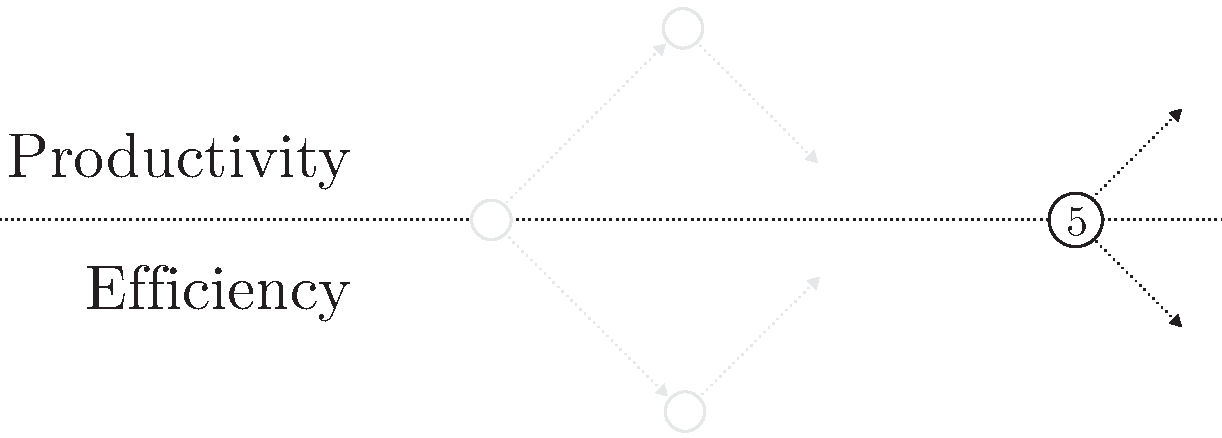
\includegraphics[width=0.6\textwidth]{../ressources/state-of-the-art-5.pdf}
\end{center}
\caption{Focus on Adoption}
\label{fig:state-of-the-art-5}
\end{figure}

\subsection{Abstraction of Tasks Organization}

\subsubsection{Compilers} \label{chapter3:software-abstraction:compilers}

\cit{It is a mistake to attempt high concurrency without help from the compiler}{R. Behren, J. Condit, E. Brewer \cite{Behren2003}}.

As soon as the incompatibility between the modules and the tasks organizations were presented, it was suggested to use a compilation approach to mitigate this incompatibility \cite{Parnas1972}.
% When showing the incompatibility between the two organization, D. Parnas  advocated conciliating the two methods using an assembler to transform the development organization into the execution organization \cite{Parnas1972}.
This section presents the state of the art to extract parallelization from sequential programs through code transformation and compilation.

\nt{read and include \cite{Catanzaro2009}}

\paragraph{Parallelism Extraction}

Extracting parallelism from a sequential implementation is a hard problem \cite{Johnston2004a}.
A compiler needs to identify the commutative operations to parallelize their executions \cite{Rinard1996,Clements2013a}.

An important work was done to parallelize loop iterations \cite{Mauras1989,Amarasinghe1995,Chen2008,Banerjee2013,Radoi2014}, particularly using the polyhedral compilation method \cite{Yuki2013,Grosser2011,Trifunovic2010,Bastoul2004}.
To improve performance gains further, some compilers identify the data-flow inside sequential programs to allow parallelism on the whole program, and not only on its loops \cite{Beck1991,Catanzaro2009,Li2012}.
Moreover, the data-flow representation and execution of a program is well suited for modern data processing applications \cite{Fernandez2014a}, as well as web services \cite{Salmito2013}.
% \nt{TODO Extract parallelism compilers from these :
% Load balanced pipeline parallelism \cite{Kamruzzaman2013}, 
% Regent \cite{Slaughter2015},
% Cilk-P, On-the-Fly Pipeline Parallelism\cite{Lee2013}
% }

% However, the limitation of modular programming regarding parallelization persists.
% In a purely functional language with immutability, higher-order functions are referentially transparent which implies commutativity hence parallelism \nt{Add reference of parallel purely functional languages}.
% \cite{Herrmann2000}
Mutable closures required for higher-order programming remains a challenge to parallelize because of the memory references shared across the program \cite{Harrison1989, Nicolay2010, Matsakis2012a}.
The next paragraphs present some improvements in parallel compilation.
% The first paragraph presents static analysis, while the second presents annotations systems.

% - Continuation-passing style parallelization compilation \cite{Harrison1989}.The interprocedural analysis and automatic parallelization of Scheme programs
% - Automatic Parallelization of Scheme Programs using Static Analysis \cite{Nicolay2010}

% - Commutativity analysis: A new analysis framework for parallelizing compilers \cite{Rinard1996}
% In this paper, they analyze commutative operations to parallelize them.
% It is novel because it isn't about parallelizing loops.
% However, it is not exactly pipeline parallelism either.

% Introducing 'Bones': a parallelizing source-to-source compiler based on algorithmic skeletons \cite{Nugteren2012}

\paragraph{Static analysis}

Compilers statically analyze the control-flow of a program to detect commutative operations \cite{Allen1970}.
The point-to analysis is a popular approach to identify side-effects \cite{Andersen1994,Jang2009,Sridharan2012,Wei2014}.
However, this analysis is not sufficient to track the dynamic control-flow of higher-order functions \cite{Shivers1991} like used in Javascript.

Another approach is the abstract interpretation of the program.
Abstract interpretation techniques are more adapted for dynamic languages like Javascript, and are successfully used for security applications \cite{Huang2004,Jovanovic2006,Yu2007,Maffeis2009a,Chudnov2015,Dolby2015}\nt{Update the citation for Dolby2015}.
It allows to statically reason on the behavior of dynamic program \cite{Maffeis2008,Smith2011,Gardner2012,Hackett2012,Raychev2013,Gardner2013,Bodin2014}.

However, static analysis techniques are too imprecise, and expensive for the performance gain to be profitable.
Instead, some compilers relies on annotations from the developers.

\paragraph{Annotations}

Some works proposed to rely on annotations from the developer to identify the commutativity of operations or the shared data structures \cite{Vandierendonck2010a,Fernandez2014a}.
Such annotations are especially relevant for accelerators such as GPUs or FPGAs, because the development effort yield huge performance improvements \cite{Tarditi2006}.
Examples of such compilers are OpenMP \cite{Dagum1998}, OpenCL \cite{Stone2010}, CUDA \cite{Nvidia2007} Cg \cite{Mark2003}, Brook \cite{Buck2004}, Liquid Metal \cite{Huang2008}.

% Bloom declarative language \ftnt{http://bloom-lang.net/}
% Blazes: Coordination analysis for distributed programs \cite{Alvaro2014}

% Livescript
% Typescript 
% Annotations, but not for parallelism.
% Asynchronism annotations should be sufficient.

\paragraph{Compilation Limitations}

The static analysis of static, low level languages like FORTRAN or C, brings performance improvements.
However for more dynamic, higher-level languages like Javascript, the static analysis is not sufficient to identify correctly the dependencies between operations to parallelize them.
And parallel compilers often fall back on relying on annotation provided by developers.
Hence, the burden of detecting commutativity of operations falls back to the developer, similarly to the platforms presented in the section \ref{chapter3:software-performance}, focusing on performance efficiency.

Alternatively, another approach is to dynamically distribute the commutative operations, and assure the communications.
The next paragraphs present runtime allowing this dynamic distribution.

\subsubsection{Runtimes} \label{chapter3:software-abstraction:runtimes}

\paragraph{Partitioned Global Address Space}

The Partitioned Global Address Space (PGAS) provides the developers with a uniform memory access on a distributed architecture.
It attempts to combine the performance efficiency of distributed memory systems, with the maintainability of shared memory systems.
Each computing node executes the same program, and provide its local memory to be shared with all the other nodes.
The PGAS platform assures the remote accesses and synchronization of memory across nodes.
Examples of implementation of the PGAS model are 
CoArray Fortran \cite{Numrich1998},
X10 \cite{Charles2005}.
Unified Parallel C \cite{El-Ghazawi2006},
Chapel\cite{Chamberlain2007},
OpenSHMEM \cite{Chapman2010}.
Kokko \cite{Edwards2012},
UPC++ \cite{Zheng2014},
RAJA \cite{Hornung2014},
ACPdl \cite{Ajima2015} and
HPX \cite{Kaiser2014,Kaiser2015}


\paragraph{Dynamic Distribution of Execution}

An interesting work following SEDA, is Leda \cite{Salmito2013,Salmito2014}.
% It follows the PCAM design methodology \cite{Foster1995} to 
It proposes a model where the stages of the pipeline are defined only by their role in the application.
% Partition $\to$ Communicate $\to$ Agglomerate $\to$ Map.
The actual execution distribution is defined automatically during deployment. % , only after the development
% blurs the distinction between the parallel organization of execution, and the modular organization of implementation.
This automation manages the execution organizations to help the developer focus on the modular organization.




\paragraph{}

Tables \ref{tab:abstraction-maintainability} and \ref{tab:abstraction-performance} presents the platforms presented in this section regarding maintainability and performance.

\AbstractionMaintainabilityTable{tab:abstraction-maintainability}

\AbstractionPerformanceTable{tab:abstraction-performance}



\subsection{Adoption Limitations}

All the platforms presented in this section come from the need to reduce the development commitment required for performance efficiency.
However, none of these platforms are highly supported by the community because they respond exclusively to industrial needs.

They are limited to scientific applications.

The balance between performance efficiency and maintainability is not sufficient for a community of passionate to gather around the platform.
The platform needs to allow the community to experiment and to start projects.
The context of web development is particularly suited to experiment and start projects.

\AbstractionAdoptionTable{tab:abstraction-performance}

\subsection{Summary}

Table \ref{tab:abstraction-summary} summarizes the characteristics of the platforms presented in this section.

\AbstractionSummaryTable{tab:abstraction-summary}

\endinput
























\section{Due Related works} \label{section:related}

To our knowledge, our work is the first to explore the transformation from continuations to Promises in Javascript, and to state the similarity between Promises and data-flow programming.
This section presents the various works related to ours.
Our work is based on the previous work on Promises and Futures~\cite{Liskov1988}, and their specifications in Javascript\footnote{\url{https://promisesaplus.com/}}\footnote{\url{https://people.mozilla.org/~jorendorff/es6-draft.html\#sec-promise-objects}}.


Because of its dominant position in the web, Javascript is recently subject to a growing interest in the field of static analysis.
We identify two teams working on static analysis for Javascript.
In the Department of Computing, Imperial College London, S. Maffeis, P. Gardner and G. Smith realised a large body of work around the static analysis of Javascript.
Their work is based around an operational semantic~\cite{Maffeis2008} to bring program understanding~\cite{Smith2011,Gardner2012,Gardner2013,Bodin2014}.
Their goal seems to revolve around security applications of this analysis~\cite{Maffeis2009,Maffeis2009a}.
In a collaboration between the programming language research groups at Aarhus University and Universität Freiburg, P. Thiemann, S. Jensen and A. Møller are working on the static analysis of Javascript.
They presented a tool providing type inference using abstract interpretation~\cite{Thiemann2005,Jensen2009,Jensen2012}.
Their goal is to improve the tools available for Javascript developers~\cite{Andreasen}.
Another example of interest for Javascript static analysis is the adaptation of the points-to analysis from L. Andersen's thesis~\cite{Andersen1994} to Javascript, by D. Jang \textit{et al.}~\cite{Jang2009} and S. Wei \textit{et al.}~\cite{Wei2014}.

The industry seems to follow the same trends.
There are some security tools based on static analysis.
We can cite for example, the company Shape Security\footnote{\url{https://shapesecurity.com/}}.
They developed \textit{Esprima}, a Javascript parser, and a serie of tools to help static analysis.
Facebook released flow\footnote{\url{http://flowtype.org/}} on 26 October 2014, a static type checker for Javascript.

Promises combine controls over the execution and the data flow.
It arrange the execution parts sequentialy and assign the result of one into the inputs of the next.
This arrangement seems similar to some works on the field of functional and data-flow programming~\cite{Johnston2004,Cohen2012,Morrison1994,Kahn1974}.
We consider it a first step in the merge of elements from the data-flow paradigm into the imperative paradigm.
The Functional Reactive Programming paradigm pushes the intrication of data and control-flow even further~\cite{Winograd-Cort2013}.

\section{Analysis}

\begin{table}[h!]
\label{maintainability-synthesis}
\small
\begin{longtabu} to \linewidth {@{} l X[l] c c c @{}}
%
% \multicolumn{3}{c}{}  & \rot{Concurrency} & \multicolumn{2}{|c}{Parallelism} \\
Model & Implementations    & \rot{Modularity} & \rot{Organic Growth} & \rot{Scalability} \\
\tabucline[.5pt]{-}
Software maintainability \\
\tabucline[.5pt]{-}
%                                                                                MOD  GRO  SCL
Imperative Programming         & C                                              & \X & \X & \X \\ \tabucline[on .5pt]{-}
Object-Oriented Programming    & C++, Java                                      & \X & \V & \X \\ \tabucline[on .5pt]{-}
Functional Programming         & Scheme, Miranda, Haskell                       & \V & \X & \X \\ \tabucline[on .5pt]{-}
Dynamic Scripting              & Javacript, Python, Ruby, Go                    & \V & \V & \X \\
\tabucline[.5pt]{-}
Concurrent Programming \\
\tabucline[.5pt]{-}
%                                                                               MOD  GRO  SCA
Event-driven programming       & Node.js, Vert.X                                & \V & \V & \X \\ \tabucline[on .5pt]{-}
Multi-threading programming    & Lock, Mutex, Semaphores, Guarded regions       & \X & \V & \V \\ \tabucline[on .5pt]{-}
Lock-free Data Structures      &                                                & \X & \V & \V \\
\tabucline[.5pt]{-}
Parallel Programming \\
\tabucline[.5pt]{-}
SPMD                           & Split-C, CRL, Composite C++                    & \X & \X & \V \\ \tabucline[on .5pt]{-}
MPMD                           & Mentat, Fortran M, Nexus                       & \X & \X & \V \\ \tabucline[on .5pt]{-}
Actor Model                    & Scala, Akka, Play, Erlang                      & \X & \X & \V \\ \tabucline[on .5pt]{-}
Data Stream System Management  & DryadLINQ \cite{Isard2007,Yu2009},%
                                 Apache Hive \cite{Thusoo2009}\ftnt{https://hive.apache.org/},%
                                 Timestream \cite{Qian2013},%
                                 Shark \cite{Xin2013}.                          & \X & \X & \V \\ \tabucline[on .5pt]{-}
Pipeline Stream Processing     & SEDA, Storm, Spark Streaming,%
                                 Spidle \cite{Consel2003},%
                                 Pig Latin \cite{Olston2008},%
                                 Piccolo \cite{Power2010},%
                                 Comet \cite{He2010},%
                                 Nectar \cite{Gunda2010},%
                                 SEEP \cite{Migliavacca2010},%
                                 Legion \cite{Bauer2012},%
                                 Halide \cite{Ragan-Kelley2013},%
                                 SDG \cite{Fernandez2014a},%
                                 Regent \cite{Slaughter2015}.                   & \X & \X & \V \\
\tabucline[.5pt]{-}
Decomposition Abstraction \\
\tabucline[.5pt]{-}
%                                                                               MOD  GRO  SCA
PGAS                           & CoArray Fortran \cite{Numrich1998},
                                 X10 \cite{Charles2005}.
                                 Unified Parallel C \cite{El-Ghazawi2006},
                                 Chapel\cite{Chamberlain2007},
                                 OpenSHMEM \cite{Chapman2010}.
                                 Kokko \cite{Edwards2012},
                                 UPC++ \cite{Zheng2014},
                                 RAJA \cite{Hornung2014},
                                 ACPdl \cite{Ajima2015},
                                 HPX \cite{Kaiser2015}                         & \V & \X & \V \\ \tabucline[on .5pt]{-}
Dynamic distribution           & LEDA                                          & \V & \X & \V \\ \tabucline[on .5pt]{-}
Parallelism extraction         & Polyhedral compiler                           & \V & \X & \V \\ \tabucline[on .5pt]{-}
Annotations                    & OpenMP \cite{Dagum1998},
                                 OpenCL \cite{Stone2010},
                                 CUDA \cite{Nvidia2007} Cg \cite{Mark2003},
                                 Brook \cite{Buck2004},
                                 Liquid Metal \cite{Huang2008}                 & \V & \X & \V \\
\tabucline[.5pt]{-}
\end{longtabu}
\caption{Synthesis of the state of the art on maintainability}
\end{table}

\endinput














\newgeometry{left=0.5cm, right=0.5cm, top=0.5cm, bottom=0.5cm}
\begin{landscape}
\begin{table}
\small
\begin{tabu} to \linewidth {@{} *2{X[c]} | *2{X[c]} | *3{X[c]} | *1{X[c]} | *2{X[c]} @{}}
%
\toprule
\multicolumn{4}{c}{}    & \multicolumn{3}{|c|}{\rot{Modularity}}                                  & \multicolumn{1}{|c|}{\rot{Concurrency}} & \multicolumn{2}{|c}{\rot{Parallelism}} \\
& & Model & Examples & \rot{Higher-Order Programming} & \rot{Closures} & \rot{Lazy Evaluation / Streams} & \multicolumn{1}{|c|}{\rot{Synchronization}} & \rot{Immutability}        & \rot{Isolation} \\
\midrule
% ✖ ⨯ ✔                                                                       HOP  CLS  LZY  SYN  IMU  ISO
\multirow{2}{*}{\rot{Section \ref{chapter3:software-maintainability:modular-programming}}} & %
\multirow{2}{*}{\rot{\parbox{2.3cm}{Modular Programming}}} & %
    Object-Oriented Programming           & C/C++, Java                       & \V & \X & \X & \X & \X & \X \\
& & Functional Programming                & Javascript                        & \V & \V & \V & \X & \X & \X \\
\midrule %
\multirow{5}{*}{\rot{Section \ref{chapter3:software-maintainability:performance}}} & %
\multirow{5}{*}{\rot{Concurrent Programming}} & %
    Event-driven                          & Node.js, Vert.X, TAME             & \V & \V & \U & \V & \X & \X \\
& & Multi-Threading                       & Lock, Mutex                       & \U & \U & \U & \V & \X & \X \\
& & Lock-Free Data Structure              &                                   & \U & \U & \U & \V & \X & \X \\
& & \multirow{2}{*}{Compilation}          & Loop parallelization              & \X & \X & \X & \V & \X & \X \\
& &                                       & CUDA, OpenCL, OpenMP ...          & \X & \X & \X & \X & \V & \V \\
\midrule %
\multirow{4}{*}{\rot{Section \ref{chapter3:software-performance:parallel-programming}}} & %
\multirow{4}{*}{\rot{\parbox{2.2cm}{Parallel Programming}}} & %
    \multirow{2}{*}{Actor Model}          & Scala, Akka, Play                 & \X & \X & \V & \X & \V & \V \\
& &                                       & Erlang                            & \V & \X & \V & \X & \V & \V \\
& & \multirow{2}{*}{Stream Processing}    & DSMS (Timestream)                 & \X & \X & \V & \X & \V & \V \\
& &                                       & Pipeline (SEDA)                   & \X & \X & \V & \X & \V & \V \\
\midrule %
\multirow{4}{*}{\rot{Section \ref{chapter3:software-performance:maintainability}}} & %
\multirow{4}{*}{\rot{\parbox{2.2cm}{Maintainability Improvements}}} & %
    Algorithmic Skeletons                 & Map Reduce ...                    & \X & \X & \V & \X & \V & \V \\
& & SOA, Microservices                    & EJB, Spring, Seneca               & \X & \X & \V & \X & \V & \V \\
& & Dynamic Distribution                  & LEDA                              & \X & \X & \V & \X & \V & \V \\
& & PGAS                                  & Chapel, X10 ...                   & \X & \X & \X & \X & \V & \V \\
\bottomrule
\end{tabu}
\caption{Synthesis of the state of the art in software design}
\end{table}
\end{landscape}
\restoregeometry

TODO

% GOTO chapter 4 - proposition
% \section{Seamless Development} \label{chapter3:objectives}
\nt{TODO title not clear enough}


\begin{center}
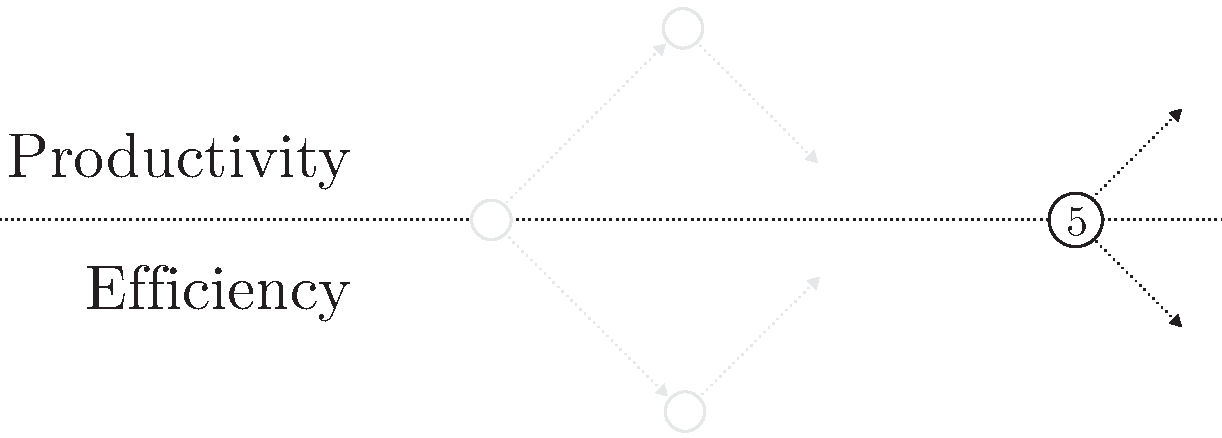
\includegraphics[width=0.6\textwidth]{../ressources/state-of-the-art-5.pdf}
\end{center}

% The objective of this thesis is to find a reconciliation of the two goals, by finding an equivalence between two approaches with different goals, in the case of streaming web applications.

The section \ref{chapter3:software-maintainability} shows that modularity and functional programming, especially higher-order programming and lazy evaluation, are the best organization to improve maintainability of an application.
This organization is best supported by a functional approach.
Indeed, higher-order programming improves readability and maintainability.
However, higher-order programming, and modular programming in general, requires the use of a global memory store.

The section \ref{chapter3:software-performance} shows that to attain scalability, an application needs to be organized to distribute its memory store into independent silos to provide isolation and immutability. Leading to multiply the exclusive accesses.
Still, many works provide this global memory store interface to developers, because it is the best way to support the modularity advocated in section \ref{chapter3:software-design}.
This incompatibility between these two organization, and their goals is responsible for the shifts operated during the life of an application.
Huge developing efforts are made to translate manually from one organization into the other, and to maintain the implementation despites its unmaintainable nature.
% when the most pressing need shift from maintainability to performance, or vice versa.

In section \ref{chapter3:objectives}, we show different tentatives to reconciles the two organizations.
Most are satisfactory for specific domains, such as the high-performance computing.
It is profitable, as the expected speedup of developing an application with an adapted programming model compensates the huge development effort.
%  where it is accepted to spend long time developing an application to use thousands of accelerators to compute heavy calculation, because the expected speedup is profitable, compared to develop an application for all these thousands accelerators.
However, none are satisfactory in the case of web applications because the need for performance is always uncertain.
The development effort is not required at the beginning, hence its cost cannot be justified.
It is only when the audience increases, often with the revenue, that the cost for the development effort can be justified.
This situation illustrate the need for a programming model reconciling the two concerns, of maintainability and performance.
% Indeed, they all are too specific, and require too much from the developer to be accepted at a large scale.

% \comment{Here a table summarizing the different approaches, and the sweet spot.}

Our objectives is to provide seamless development.
3.1 shows that modularity is not scalable but needed.
But compilation can help to get scalable.
3.2 shows that parallelism is not maintainable (no Higher-Order Programming, no lazy evaluation, so no good glue between modules)
But good developers can maintain double representation.
With help from an equivalence or a \textit{compiler} most developers could develop using this double representation, and seamlessly achieving parallelism and maintainability.

\begin{table}
\begin{tabular}{l|l|l|l}
             & Maintainability         & Performance           & Both\\\hline
General      & Functional Programming  & Message-passing       & Loop parallelization\\
Web          & Javascript              & Pipeline architecture & ø
\end{tabular}
\caption{Summary of the state of the art}
\label{tab:chapter3:objectives:summary}
\end{table}

\nt{integrate these paragraphs after the next section}
Our objectives is to find an equivalence between these two organization, specifically for the case of web applications.
To do so, we focus on the Javascript programming language, and specifically, the node.js interpreter.
\nt{TODO not clear}
As explained in the end of chapter \ref{chapter2}, the execution model of Javascript is similar to a pipeline.
We intend to split a node.js application into a parallel pipeline of stages.

The contribution of this thesis is organized in two chapters, as illustrated in figure \ref{fig:chapter3:objectives:roadmap}.
In chapter \ref{chapter4} I present the extraction of a pipeline of operations from a Javascript application.
I show that such pipeline is similar to the one exposed by Promises, and I propose a simpler alternative to the latter called Dues.
However, these operations still require a global memory for coordination so they are not executed in parallel.
In chapter \ref{chapter5}, we present the isolation of the operations into isolated containers called Fluxions. 

\begin{figure}[h!]
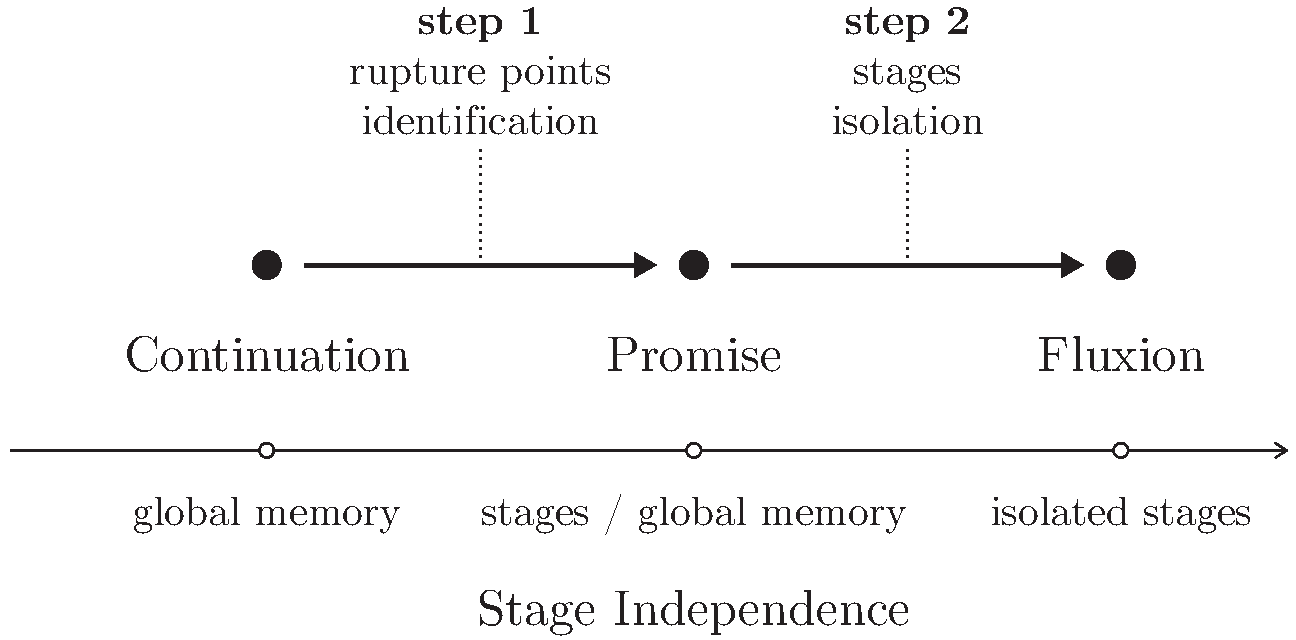
\includegraphics[width=1\textwidth]{../ressources/roadmap.pdf}
\caption{Roadmap for this work}
\label{fig:chapter3:objectives:roadmap}
\end{figure}

\begin{center}
\rule{3cm}{0.4pt}
need integration
\rule{3cm}{0.4pt}
\end{center}

We show that there is no languages that features higher-order functions to improve modularity, a common memory store easy to develop with, but at the same time provides scalable concurrency.

We aim at filling this gap, and for a concrete example, focus our work on the Javascript programing language.
Indeed, Javascript features higher-order functions, is highly-used in concurrent context, but lacks scalable concurrency.








\subsection{Equivalence}

\subsubsection{Rupture Point}

The execution of the pipeline architecture is well delimited in isolated stages.
Each stage has its own thread of execution, and is independent from the others.
On the contrary, the code of the event-loop is linear because of the continuation passing style and the common memory store.
% The message passing linking the callbacks is transparently handled by the event-loop.
However, the execution of the different callbacks are as distinct as the execution of the different stages of a pipeline.
The call stacks of two callbacks are distincts.
Therefore, an asynchronous function call represents the rupture between two call stacks.
It is a rupture point, and is equivalent to a data stream between two stages in the pipeline architecture.

Both the pipeline architecture and the event-loop present these rupture points.
The detection of rupture points allows to map a pipeline architecture onto the implementation following the event-loop model.
To allow the transformation from one to the other, this thesis studies the possibility to detect rupture points, and to distribute the global memory into the parts defined by these rupture points.
The detection of rupture points is addressed in chapter \ref{chapter4}.

\subsubsection{Invariance}

% This transformation is important on two points.
% The conservation of the invariance.
% The equivalence between the coordinations.

The transformation should preserve the invariance as expressed by the developer to assure the correctness of the execution.
The partial ordering of events in a system, by opposition to total ordering, is sufficient to assure this correctness.
% This result was used by Lamport to prove the correctness of distributed systems.
The global memory is a way to assure the total ordering of events, and the message passing coordination is a way to assure partial ordering of events.
Therefore, to assure the correctness of the execution of a system, the state coordination with a global memory is equivalent to message passing coordination.
And it is possible, at least for some rupture points, to transform the global memory coordination into message passing while conserving the correctness of execution.

In order to preserve the invariance assured by the event-loop model after the transformation, each stage of the pipeline needs to have an exclusive access to memory.
The global memory needs not to be split into parts and distributed into each of the stages.
To assure the missing coordinations assured by the shared memory between the stages, the transformation should provide equivalent coordination with message passing.
The isolation and replacement of the global memory is fully address in chapter \ref{chapter5}

% The invariance holds for the whole memory during the execution of each callback.
% As I explained in the previous section, this invariance is required to allow the concurrent execution of the different tasks.
% On the other hand, the invariance is explicit in the pipeline architecture, as all the stages have isolated memories.
% The coordination between these isolated process is made explicit by the developer through message passing.

% I argue that the state coordination between the callbacks requireing a global memory could be replaced by the message passing coordination used manually in the pipeline architecture.
% I argue that not all applications need concurrent access on the state, and therefore, need a shared memory.
% % Specifically, I argue that each state region remains roughly local to a stage during its modification.
% \nt{TODO review that, I don't know how to formulate these paragraphs. Identify the state and the data in the global memory.}

% \subsubsection{Transformation}

% This equivalence should allow the transformation of an event loop into several parallel processes communicating by messages.
% In this thesis, I study the static transformation of a program, but the equivalence should also hold for a dynamic transformation.
% I present the analyzis tools I developed to identify the state and the data from the global memory.




%-----------------------------------------------------------------------------%
                                    \endinput
%-----------------------------------------------------------------------------%


Some links I NEED to put :
--------------------------

https://glyph.twistedmatrix.com/2014/02/unyielding.html
http://calculist.org/blog/2011/12/14/why-coroutines-wont-work-on-the-web/

Transitions :
  - Linkedin - http://engineering.linkedin.com/architecture/brief-history-scaling-linkedin
  - Facebook - https://www.cs.princeton.edu/events/event/evolution-software-architecture-facebook / http://www.infoq.com/presentations/Evolution-of-Code-Design-at-Facebook
  - ... 

https://medium.com/@benorama/the-evolution-of-software-architecture-bd6ea674c477

https://en.wikipedia.org/wiki/Dataflow
https://en.wikipedia.org/wiki/Real-time_computing
https://en.wikipedia.org/wiki/Partitioned_global_address_space
https://en.wikipedia.org/wiki/SPMD

Albert Cohen
https://scholar.google.com/citations?user=MkKZKAMAAAAJ&hl=en

+ Paul Feautrier (Tutor of A. Cohen)


Similar problem :
http://2015.splashcon.org/event/splash2015-splash-i-lindsey-kuper-talk
http://www.cs.indiana.edu/~lkuper/papers/lindsey-kuper-dissertation.pdf

PJS was abandoned :
https://groups.google.com/forum/#!topic/mozilla.dev.tech.js-engine/H-YEsejE6DA
https://bugzilla.mozilla.org/show_bug.cgi?id=1117724

See parallel JS for further work (maybe) :
http://smallcultfollowing.com/babysteps/blog/2014/04/24/parallel-pipelines-for-js/

Some chunks I might find useful later :
---------------------------------------

A good example of declarative sentence in everyday world : in case of fire, 
the elevators don't work -> you understand that you need to take the stairs.